\vspace{-1em}
\section{Evaluation}
\label{sec:eval}
%\vspace{-0.5em}
 We evaluate the efficacy of our dynamic parallelotope bundle strategies with our tool, \emph{Kaa} \cite{kim2020kaa}. Kaa is written in Python and relies on the \emph{numpy} library for matrix computations, \emph{sympy} library for all symbolic subsitution, and \emph{scipy}, \emph{matplotlib} for plotting the reachable sets and computing the volume for lower-dimensional systems. The optimization procedure for finding the direction offets is performed through the \emph{Kodiak} library. Finally, parallelization of the offset calculation procedures is implemented through the \emph{multiprocessing} module. To estimate volume of reachable sets, we employ two techniques for estimating volume of individual parallelotope bundles. For systems of dimension fewer than or equal to three, we utilize scipy.spatial library's Convex hull routine.
 These routines are esstentially Python wrappers around their corresponding \emph{QHull} procedures. For higher-dimensional systems, we employ the volume of the tightest enveloping box around the intersection of the parallelotopes.
 The dimensions of this box are easily calculated through linear programming. The total volume estimate of the reachable set will be the sum of all the computed bundles' volume estimates.

 %For two-dimensional models, note that there are only five non-trivial templates. The trivial template here refers to the initial box which is defined exactly the axis-aligned directions. Refer to the non-axis aligned templates. At each every time, pca. lin app directions to
\vspace{-1em}
\subsubsection{Model Dynamics}
For benchmarking, we select six non-linear models with polynomial dynamics. Many of these models are also implemented in \emph{Sapo} \cite{dreossi2017sapo}, a previous tool exploring reachability analysis with {\bf static} parallelotope bundles. In these cases, we directly compare the performance of our dynamic strategies with the static parallelotopes defined in Sapo. To provide meaningful comparisions, we set the number of dynamic parallelotopes to be equal to the number of static ones excluding the initial box. Here, {\bf diagonal directions} are defined to be the vectors created by adding and subtracting distinct pairs of all unit axis-aligned vectors from each other. By {\bf diagonal parallelotopes}, we refer to parallelotopes which are defined only by axis-aligned and diagonal directions. Similarly, {\bf diagonal parallelotope bundles} are parallelotope bundles which solely consists of diagonal parallelotopes. Sapo primarily utilizes {\bf static diagonal parallelotope bundles} to perform its reachability computation.
Note that the initial box, which is defined only through the axis-aligned directions, is contained in every bundle.
For our experiments, we are concerned with the effects of additional static or dynamic parallelotopes added alongside the initial box. We refer to these parallelotopes as {\bf non-axis-aligned parallelotopes}.

%Maybe mention something about role of diagonal templates in program verfication here.
\begin{example}
In two dimensions, $\mathbb{R}^2$, we have the two unit axis-aligned directions, $[1,0]^T, [0,1]^T$. The diagonal directions will then

\[ [1,1]^T, \; [1,-1]^T\]
Consequently, the diagonal parallelotopes will be precisely be defined by unique pairs of these directions, giving us a total ${4 \choose 2} = 6$ diagonal parallelotopes.
% Similarly, in $\mathbb{R}^3$, we have three unit axis-aligned directions $[1,0,0]^T, [0,1,0]^T,[0,0,1]^T$. Calculating the diagonal directions yields the following directions:
% \[ [1,1,0]^T, \; [1,-1,0]^T, \; [1,0,1]^T,\;  [1,0,-1]^T,\;  [0,1,1]^T, \; [0,1,-1]^T \]
% Thus, there are ${9 \choose 3} = 84$ diagonal parallelotopes.
%
% Note that for both examples, we do not consider the directions' negative counterparts since we define parallelotopes use both the positive and negative counterparts of a its chosen directions.
%
% For two dimensions, the non-axis-aligned parallelotopes would be all parallelotopes excluding the one defined by directions $[0,1]^T, [1,0]^T$. In particular, there are 5 non-axis-aligned diagonal parallelotopes.
\end{example}
Table \ref{tab:modeldyns} summarizes five standard benchmarks used for experimentation. The last seven-dimensional model COVID supermodel is explained in the subsequent subsection below.

\vspace{-1em}
\begin{table}[h!]
%\hspace{-5em}
  \centering
\begin{tabular}{|p{1.5cm}|c|p{1.5cm}|c|c|p{5cm}|}
\hline
Model & Dimension & Parameters & \# steps & $\Delta$ & \hspace{1.5cm}Initial Box \\
\hline
Vanderpol & 2 & - & 70 steps & 0.08 & $x \in [0,0.1], y \in [1.99,2]$ \\
\hline
Jet Engine& 2 & - & 100 steps & 0.2 & $x \in [0.8,1.2], y \in [0,8,1.2]$ \\
\hline
Neuron \cite{fitzhugh1961impulses}& 2 & - & 200 steps & 0.2 & $x \in [0.9,1.1], y \in [2.4,2.6]$ \\
\hline
SIR& 3 & $\beta=0.05$ \newline $\gamma=0.34$ & 150 steps & 0.1 & $s \in [0.79,0.8], i \in [0.19,0.2], r = 0$ \\
\hline
Coupled \newline Vanderpol & 4 & - & 40 steps & 0.08 & $x1 \in [1.25, 2.25], y1 \in [1.25, 2.25]$ \newline $x2 \in [1.25, 2.25], y2 \in [1.25, 2.25]$ \\
\hline
COVID & 7 & $\beta=0.05$ \newline $\gamma=0.0$ \newline $\eta=0.02$ & 200 steps & 0.08 & Stated Below\\
\hline
\end{tabular}
\caption{Benchmark models and relevant information}
\label{tab:modeldyns}
\end{table}

\vspace{-2em}
\noindent \textbf{COVID Supermodel:}
%
We further benchmark our dynamic strategies with the recently introduced COVID supermodel \cite{ansumali2020modelling}, \cite{indiansuper2020supermodel}. This model is a modified SIR model accounting for the possibility of \emph{asymptomatic} patients. These patients have the ability to infect susceptible members with a fixed probability. The following dynamics account for this new group and its interactions with the traditional groups found in the SIR model. The continuous dynamics given in \cite{indiansuper2020supermodel} are discretized through the Euler method.

\begin{align}
  \begin{split}
   S_A & = S_A  -(\beta S_A(A+I))\cdot \Delta \\
   S_I & = S_I  -(\beta S_I (A + I))\cdot \Delta \\
   A & = A + (\beta S_I(A+I) - \gamma I)\cdot \Delta \\
   I & = I + (\beta S_I (A+I) - \gamma I)\cdot  \Delta \\
   R_A & = R_A + (\gamma A)\cdot \Delta \\
   R_I & = R_I + (\gamma I)\cdot \Delta \\
   D & = D + (\eta I)\cdot \Delta
  \end{split}
\end{align}
where the variables denote the fraction of a population of individuals designated as \emph{Susceptible Transition to Asymptomatic $(S_A)$}, \emph{Susceptible Transition to Infected $(S_I)$}, \emph{Asymptomatic (A)}, \emph{Symptomatic (I)}, \emph{Removed from Asymptomatic $(R_A)$}, \emph{Removed from Symptomatic $(R_I)$}, and \emph{Deceased (D)}. We choose the parameters ($\beta = 0.25, \gamma=0.02, \eta=0.02$) where $\beta$ is the average probablity of infection, $\gamma$ is the average removal rate, and $\eta$ is the average mortality rate. The parameters are set based on figures shown in \cite{ansumali2020modelling} for the USA. The discretization step is chosen to be $\Delta = 0.1$ and the initial box is set to be following dimensions: $S_A  \in [0.69, 0.7], \, S_I \in [0.09, 0.1], \, A \in [0.14, 0.15], \, I \in [0.04, 0.05], \, R_A  = 0,\, R_I  = 0, \, D  = 0$.

\subsubsection{Accuracy of Dynamic Strategies}
The results of testing our dynamic strategies against static ones are summarized in Table~\ref{tab:voltable}. For models previously defined in Sapo, we set the static parallelotopes to be exactly those found in Sapo.
If a model is not implemented in Sapo, we simply use the static parallelotopes defined in a model of equal dimension. To address the unavailability of a four-dimensional model implemented in Sapo, we sampled random subsets of five static non-axis-aligned parallelotopes and chose the flowpipe with smallest volume.
%
% As justifiction for this scheme, we wish to remark the time required in testing all possible subsets of diagonal parallelotopes.
%
A cursory analysis shows that the number of possible templates with diagonal directions grows with $O(n^n)$ with the number of dimensions and hence an exhaustive search on optimal template directions is impossible.

% are $2{n \choose 2}$ diagonal directions for an $n$-dimensional system, giving a total of $n + 2 {n \choose 2}$ axis-aligned and diagonal directions. Thus, there are ${n + 2 {n \choose 2} \choose n} = {n^2 \choose n}$ possible diagonal parallelotopes for an $n$-dimensional system. This explosive growth in search space size compelled us to proceed by sampling the search space instead.

From our experiments, we conclude there is no universal optimal ratio between the number of dynamic parallelotopes defined by PCA and Linear Approxiation directions which perform well on all benchmarks. In Figure \ref{fig:PCALinAppRatio}, we demonstrate two cases where varying the PCA/LinApp ratio imparts differing effects on the reachable set.  Observe that using parallelotopes defined by Linear Approximation directions is more effective than those defined by PCA directions in the Vanderpol model whereas the Neuron model shows the opposite trend.

\begin{figure}[h!]
\begin{subfigure}{0.5\textwidth}
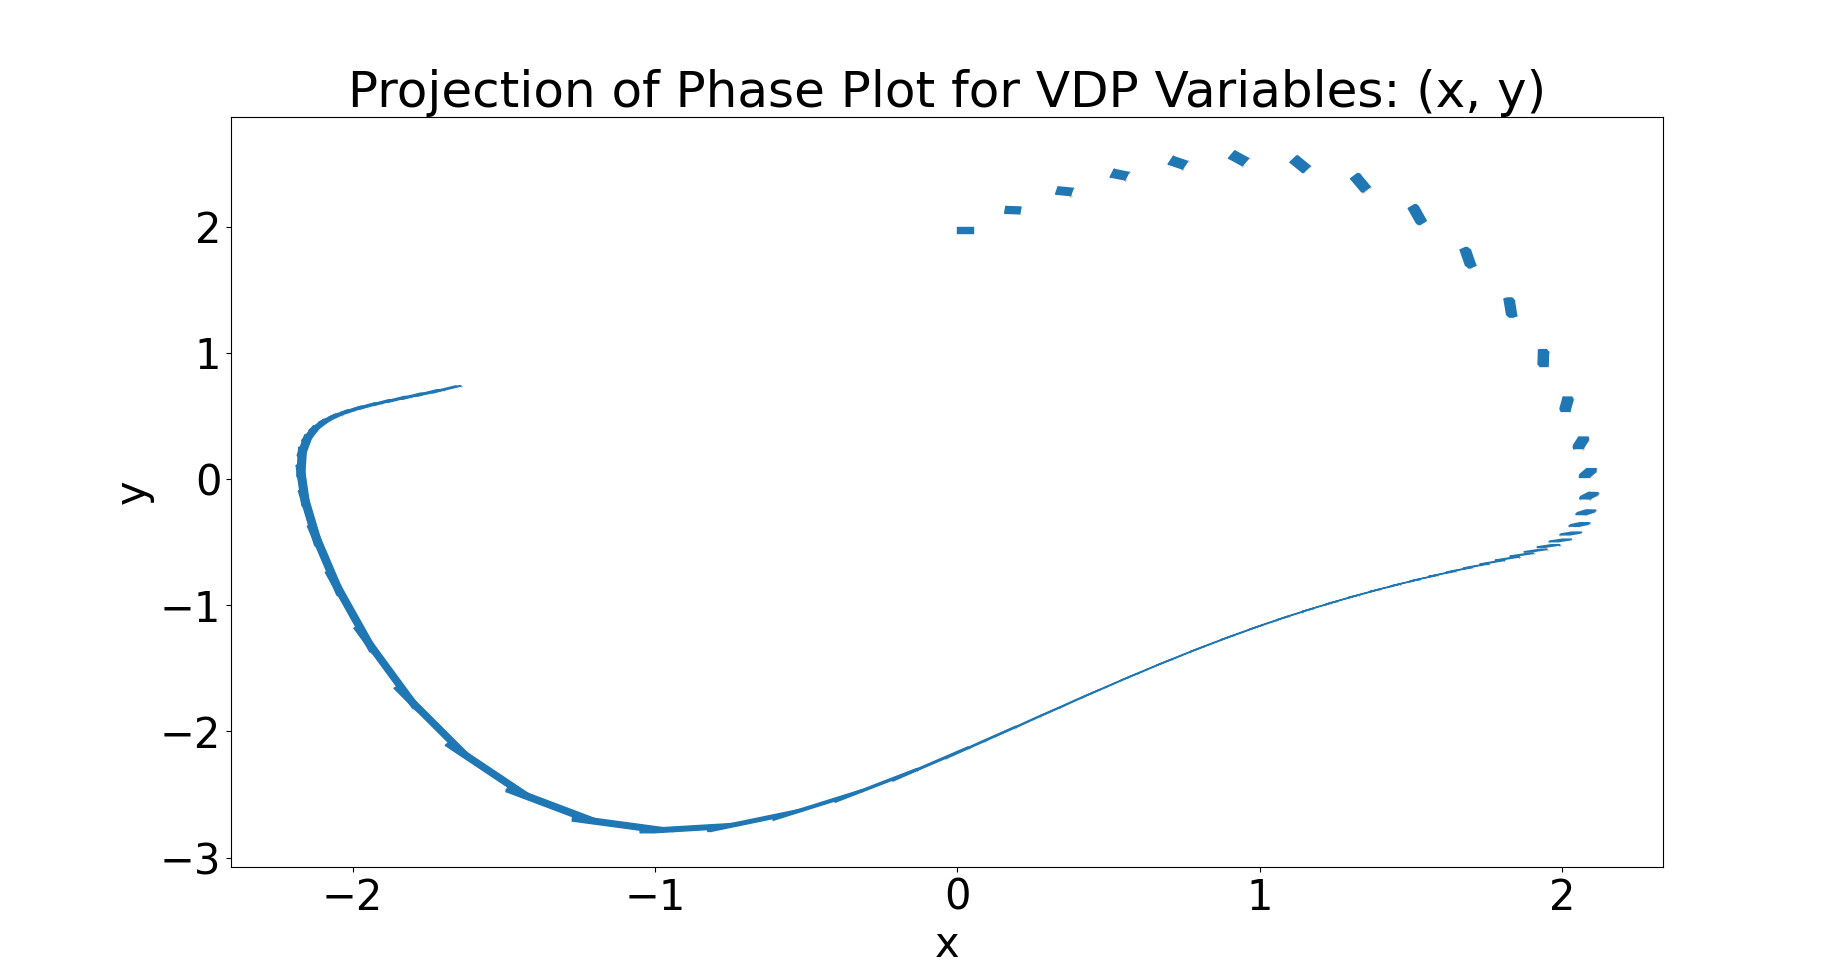
\includegraphics[width=\textwidth]{figures/PhasePlots/VDP_5Lin_.png}
\caption{5 Lin}
\end{subfigure}%
\begin{subfigure}{0.5\textwidth}
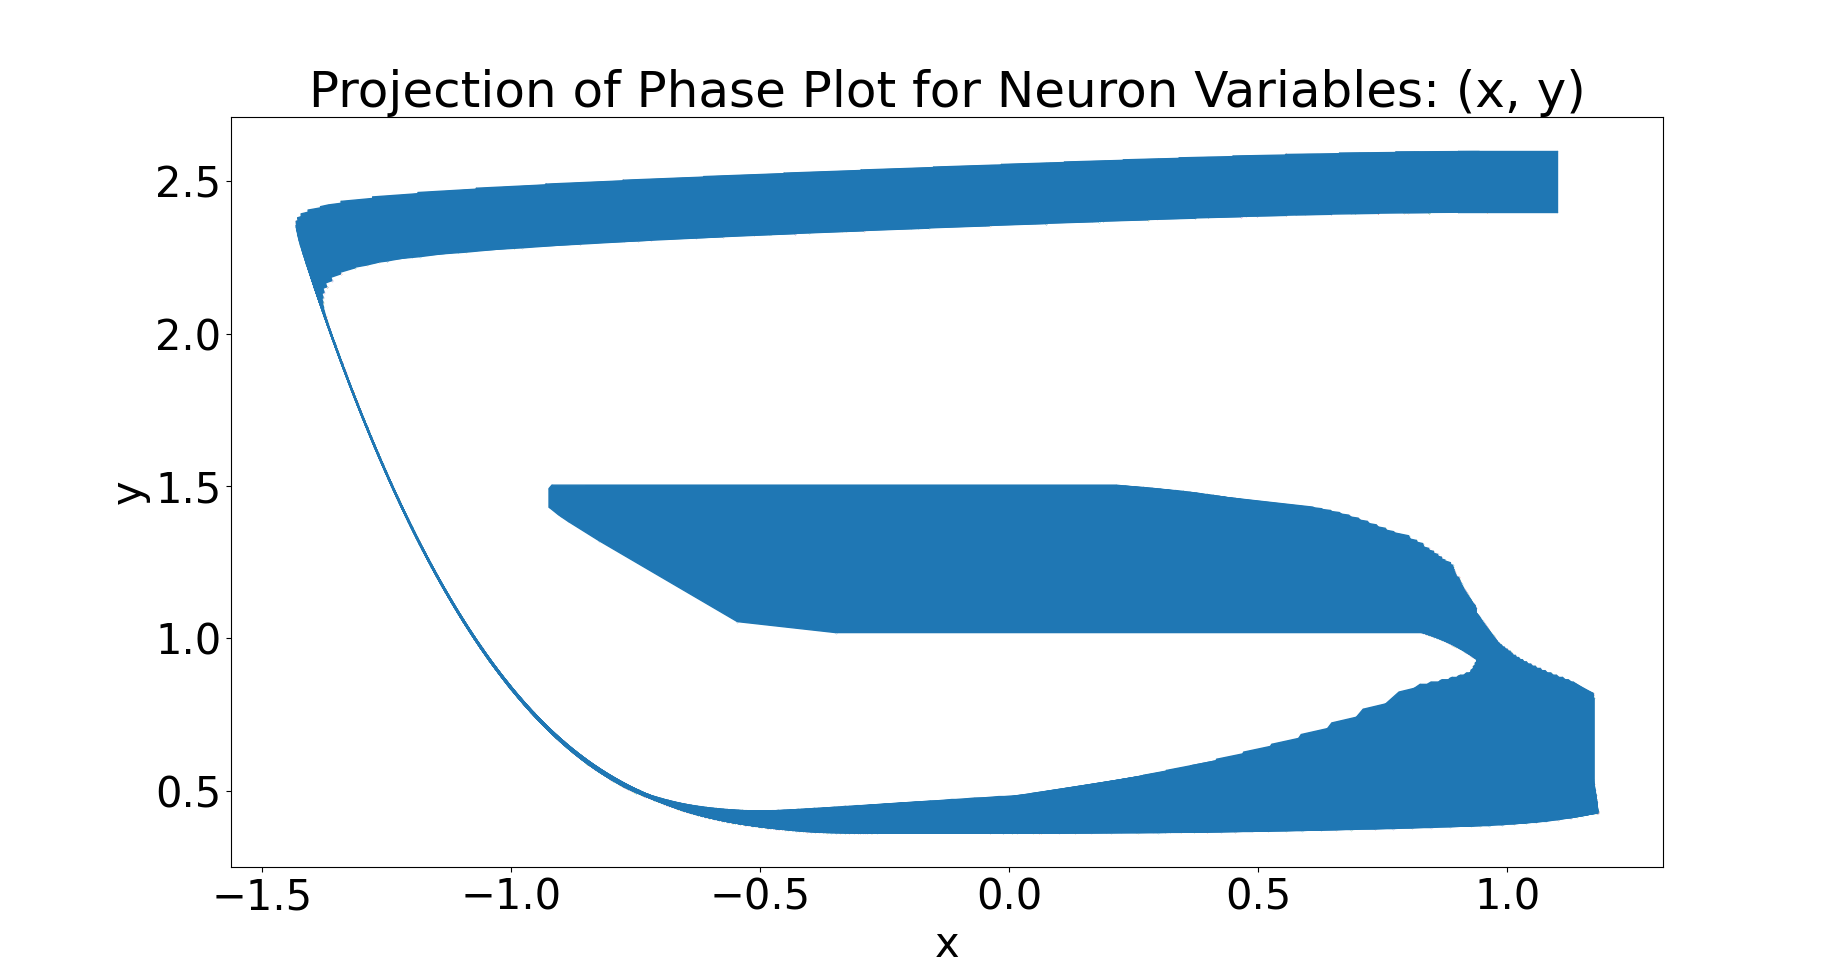
\includegraphics[width=\textwidth]{figures/PhasePlots/Neuron_1PCA5Lin_.png}
\caption{1 PCA 5 Lin}
\end{subfigure}%

\begin{subfigure}{0.5\textwidth}
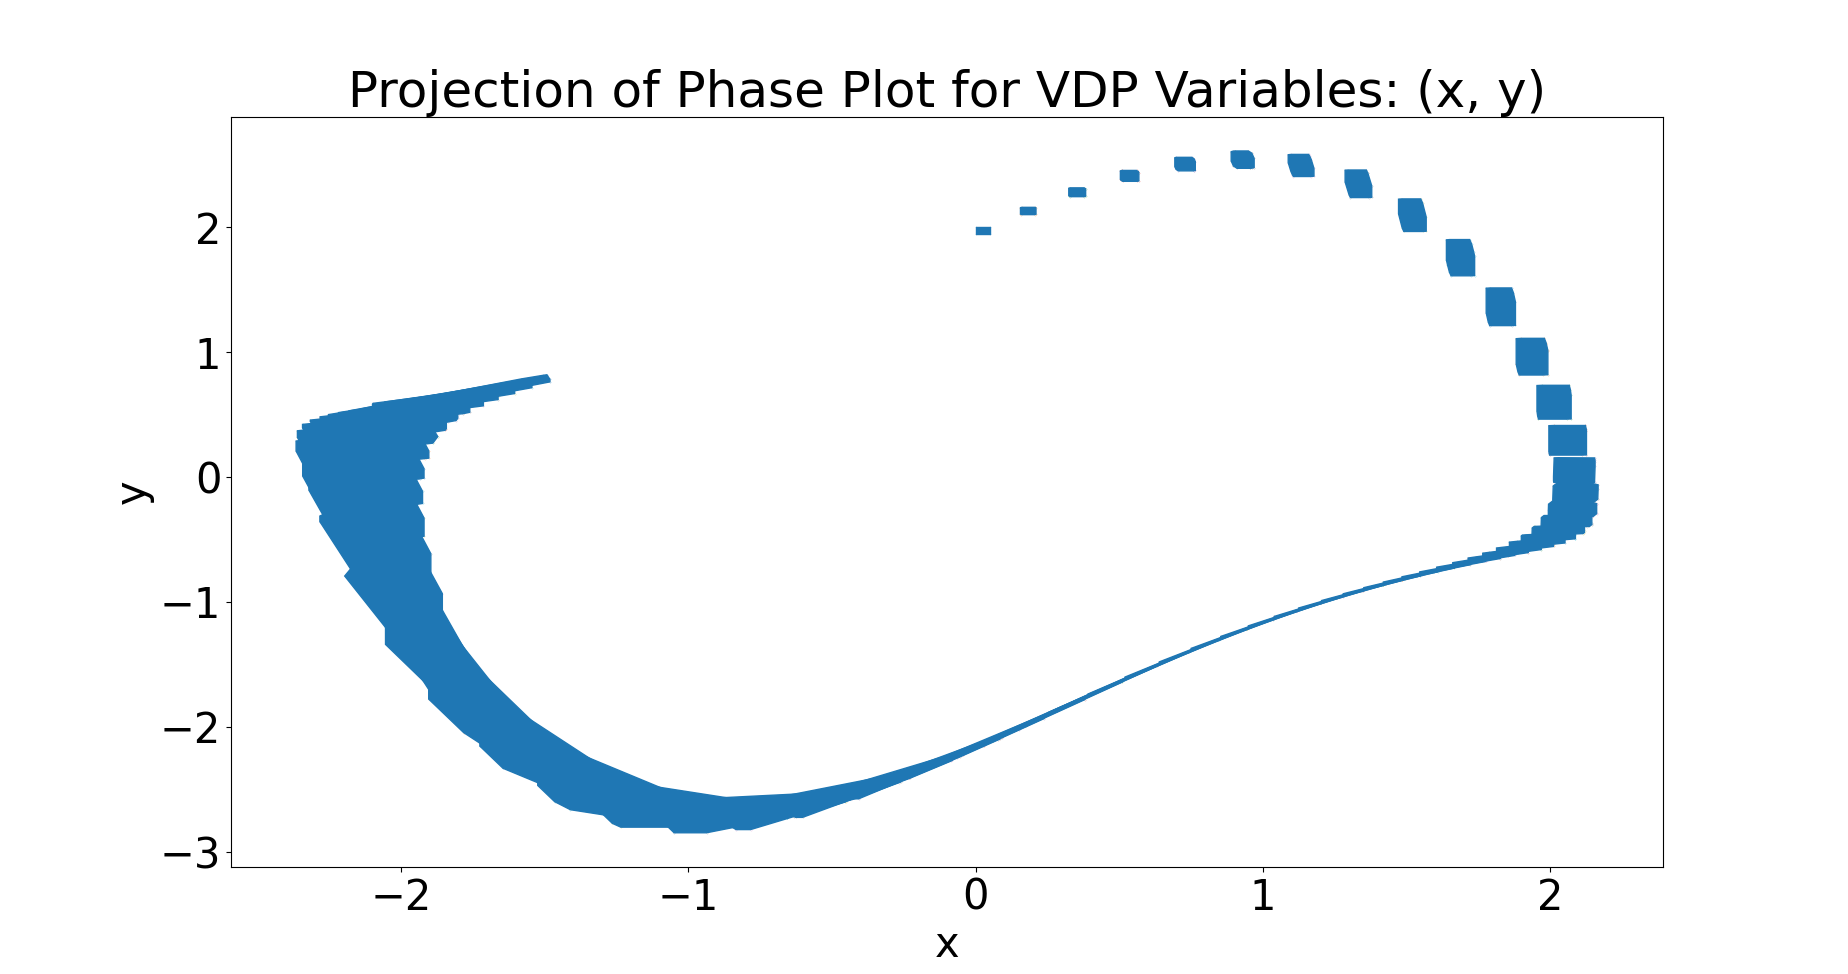
\includegraphics[width=\textwidth]{figures/PhasePlots/VDP_5PCA_.png}
\caption{5 PCA}
\end{subfigure}%
\begin{subfigure}{0.5\textwidth}
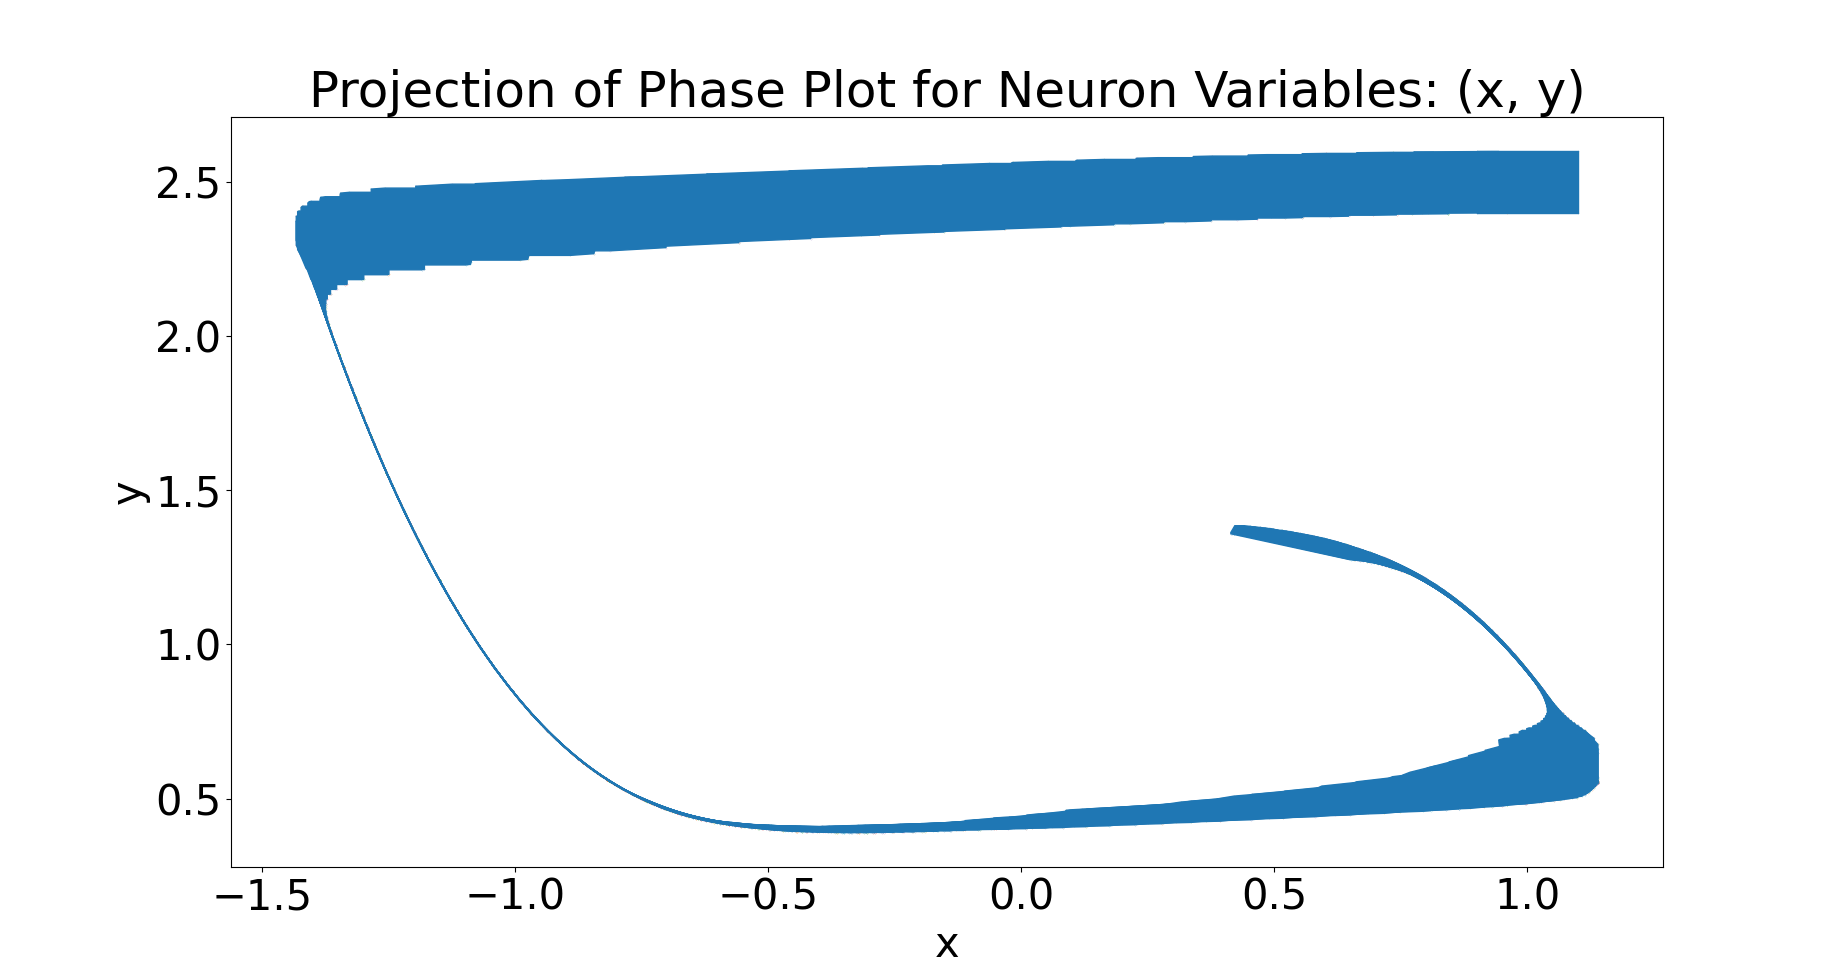
\includegraphics[width=\textwidth]{figures/PhasePlots/Neuron_5PCA1Lin_.png}
\caption{5 PCA 1 Lin}
\end{subfigure}

\begin{subfigure}{0.5\textwidth}
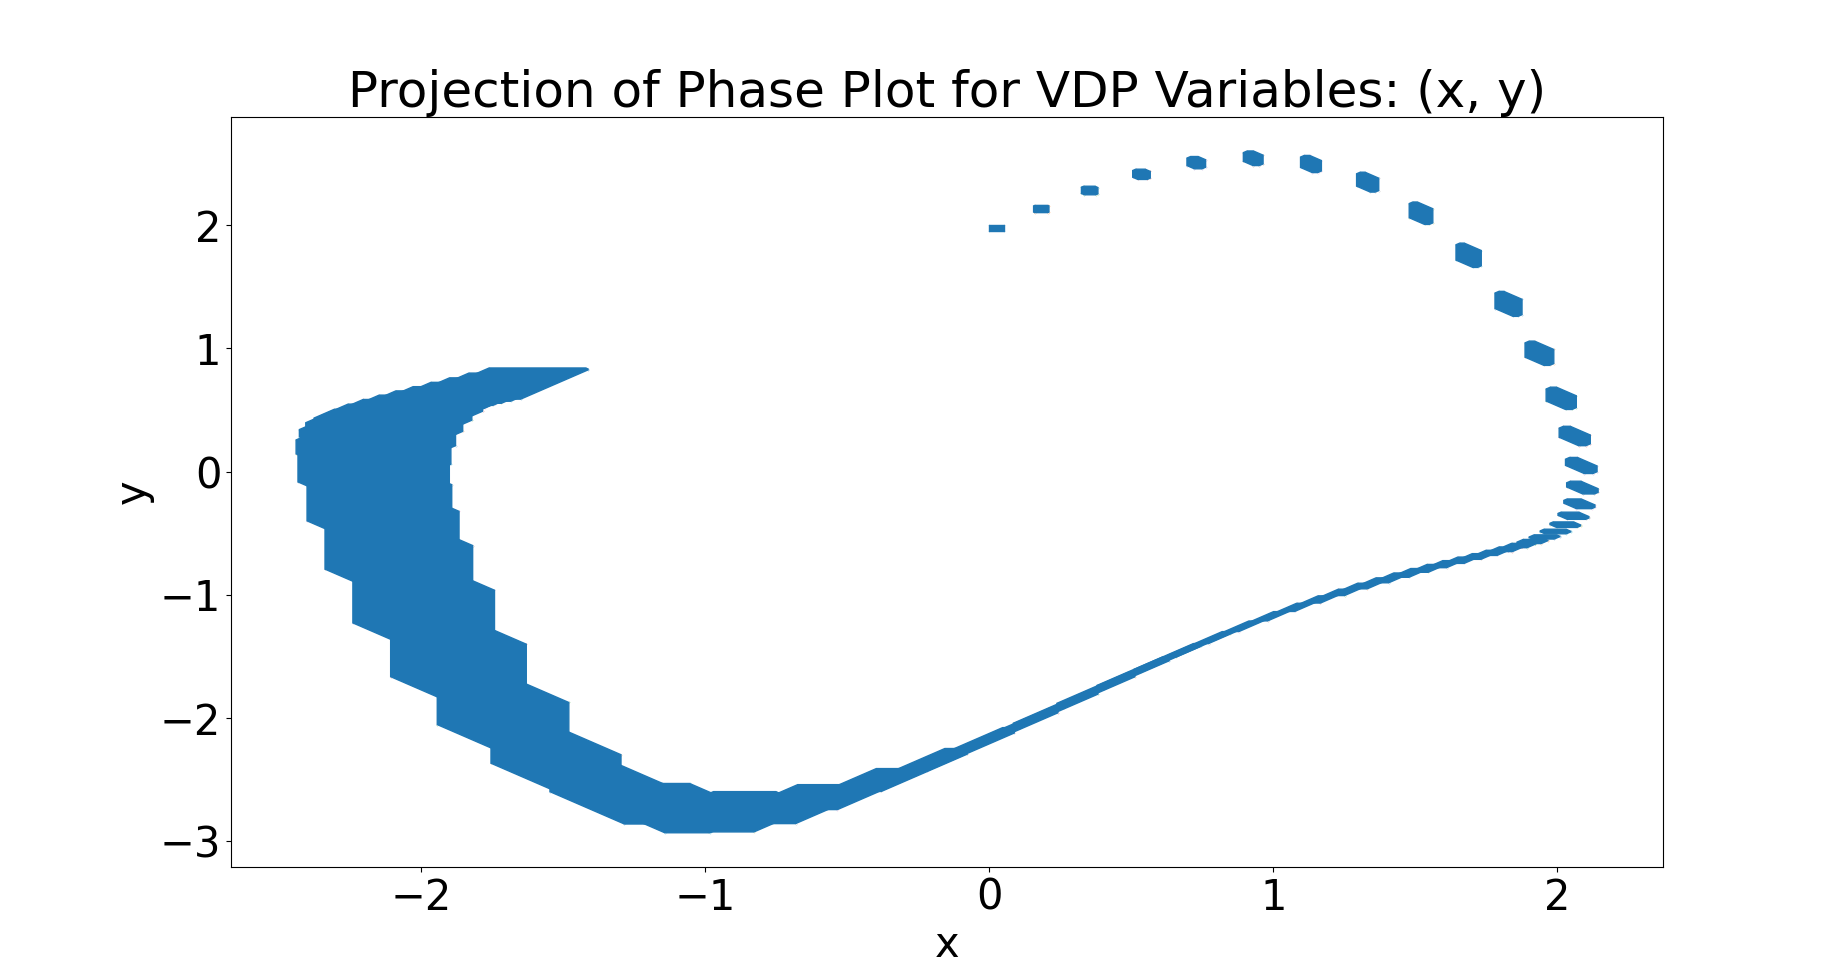
\includegraphics[width=\textwidth]{figures/PhasePlots/VDP_Sapo_.png}
\caption{Sapo}
\end{subfigure}%
\begin{subfigure}{0.5\textwidth}
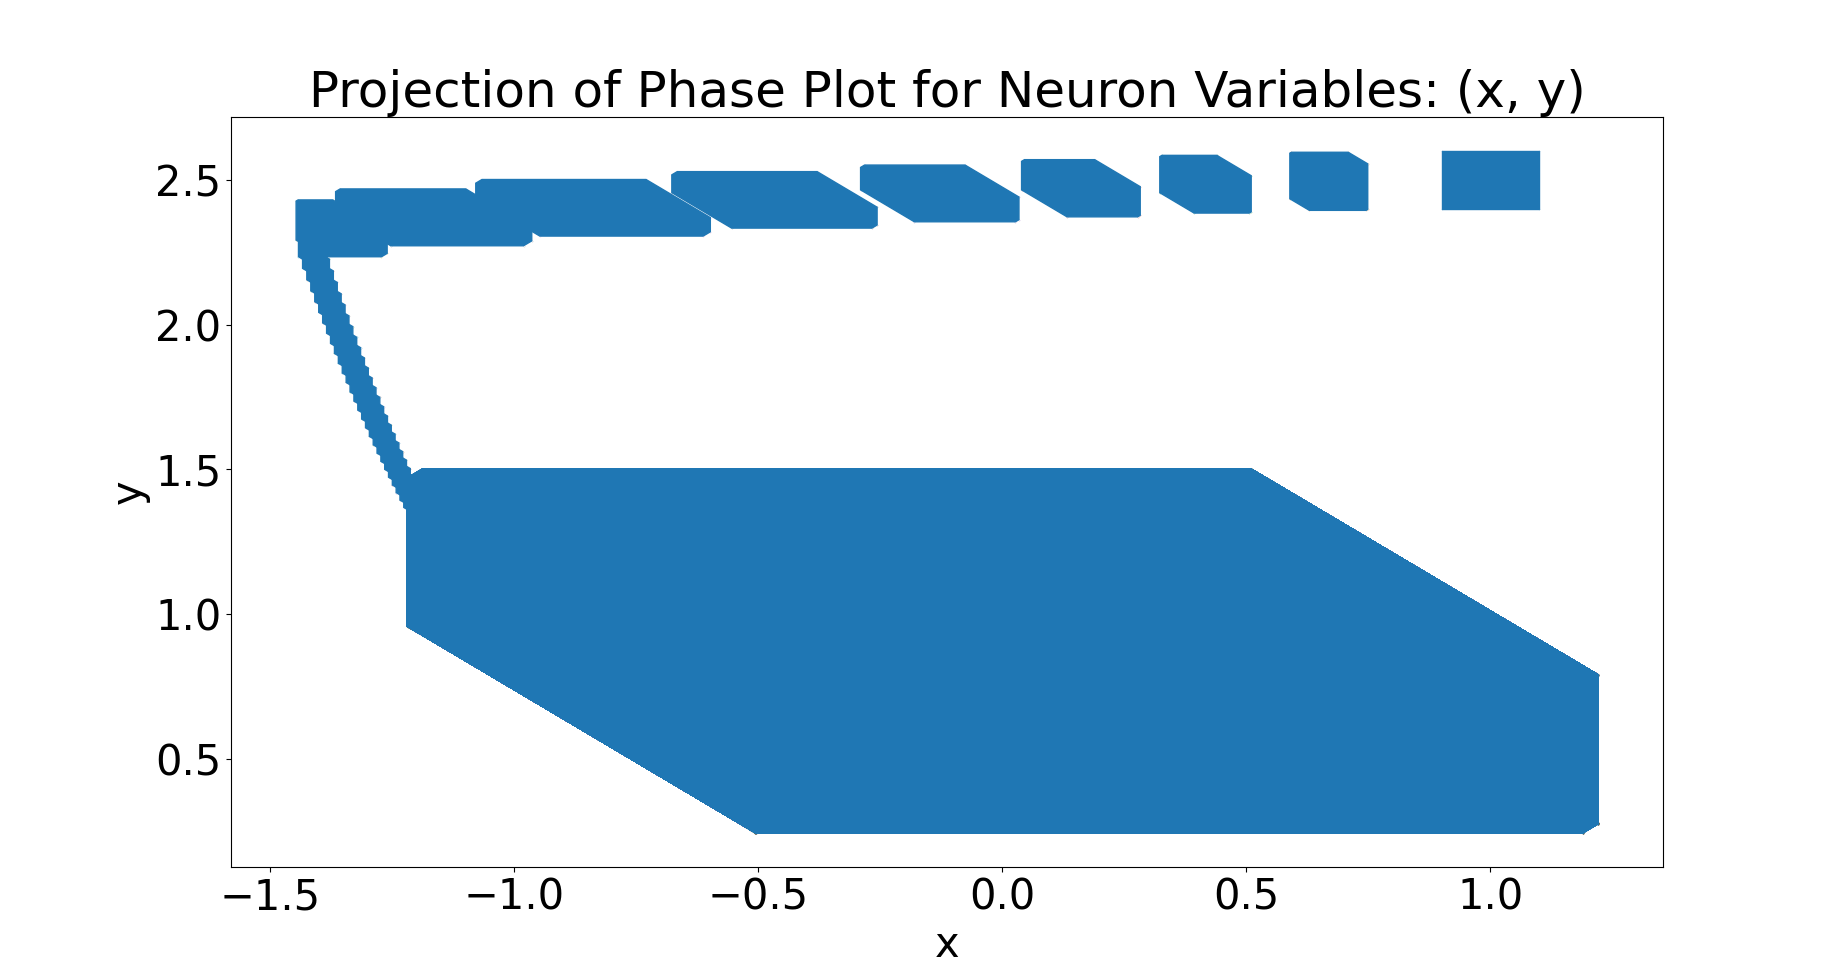
\includegraphics[width=\textwidth]{figures/PhasePlots/Neuron_Sapo_.png}
\caption{Sapo}
\end{subfigure}
\caption{Effect of varying ratio between the number of PCA and Linear Approximation parallelotopes. The Vanderpol (left) and the FitzHugh-Nagumo Neuron (right) phase plots are shown to illustrate differing effects of varying the PCA/LinApp ratio. The initial set for the Vanderpol model is set to $x \in [0,0.05], \, y \in [1.95,2]$}
\label{fig:PCALinAppRatio}
\end{figure}

\vspace{-1em}
\subsubsection{Performance under Increasing Initial Sets}
A key advantage of our dynamic strategies is the improved ability to control the wrapping error naturally arising from larger initial sets. Figure \ref{fig:InitVolReachComp} presents charts showcasing the effect of increasing initial sets on the total flowpipe volume. We vary the initial box dimensions to gradually increase the box's volume. We then plot the total flowpipe volume after running the benchmark. The same initial boxes are also fed as input into computation using only static parallelotopes borrowed from Sapo. The number of parallelotopes defined by PCA and Linear Approximation directions were chosen based on best performance as seen in Table \ref{tab:voltable}. We remark that our dynamic strategies perform better than static ones in controlling the total flowpipe volume as the initial set becomes larger. On the other hand, the performance of static parallelotopes tends to degrade rapidly as we increase the volume of the initial box.

\subsubsection{Performance against Random Static Templates}
We additionally benchmark our dynamic strategies against static random parallelotope bundles. We sample such parallelotopes in $n$ dimensions by first sampling a set of $n$ directions uniformly on the surface of the unit $(n-1)$-sphere, then defining our parallelotope using these sampled directions. We sample twenty of these parallelotopes for each trial and average the total flowpipe volumes. As shown in Figure \ref{fig:RanStaticStratComp}, our best-performing dynamic strategies consistently outperform static random strategies for all tested benchmarks.

\vspace{-1em}
\section{Conclusions}
In this paper we investigated two techniques for generating templates dynamically, first using linear approximation of the dynamics, and second using PCA.
%
We demonstrated that these techniques improve the accuracy of reachable set by an order of magnitude when compared to static or random template directions.
%
We also observed that both these techniques improve the accuracy of the reachable sets for different benchamrks.
%
In future, we intend to investigate Koopman linearization techniques for computing the template directions~\cite{bak2021reachability}.

\begin{table}[h!]
\hspace{1em}
\begin{subtable}[h]{0.45\textwidth}
     \centering
     \begin{tabular}{|c|c|}
     \hline
     Strategy & Total  Volume \\
     \hline\
     5 LinApp & 0.227911 \\
     \hline
     1 PCA, 4 LinApp& 0.225917 \\
     \hline
     2 PCA, 3 LinApp & 0.195573 \\
     \hline
     {\bf 3 PCA, 2 LinApp} & {\bf 0.188873} \\
     \hline
     4 PCA, 1 LinApp & 1.227753\\
     \hline
     5 PCA & 1.509897 \\
     \hline
     5 Static Diagonal(Sapo) & 2.863307  \\
     \hline
    \end{tabular}
    \caption{Vanderpol}
    \label{tab:vdpvol}
 \end{subtable}\hspace{1em}
 \begin{subtable}[h]{0.45\textwidth}
      \centering
      \begin{tabular}{|c|c|}
      \hline
      Strategy & Total  Volume \\
      \hline
      5 LinApp & 58199.62 \\
      \hline
      1 PCA, 4 LinApp & 31486.16 \\
      \hline
      {\bf 2 PCA, 3 LinApp} & {\bf 5204.09}\\
      \hline
      3 PCA, 2 LinApp & 6681.76 \\
      \hline
      4 PCA, 1 LinApp& 50505.10 \\
      \hline
      5 PCA  & 84191.15 \\
      \hline
      5 Static Diagonal (Sapo) & 66182.18  \\
      \hline
     \end{tabular}
     \caption{Jet Engine}
     \label{tab:enginevol}
  \end{subtable}

  \hspace{1em}
  \begin{subtable}[h]{0.45\textwidth}
       \centering
       \begin{tabular}{|c|c|}
       \hline
       Strategy & Total  Volume \\
       \hline
       5 LinApp  & 154.078\\
       \hline
       1 PCA, 4 LinApp  & 136.089\\
       \hline
       2 PCA, 3 LinApp  & 73.420\\
       \hline
       {\bf 3 PCA , 2 LinApp } & {\bf 73.126} \\
       \hline
       4 PCA, 1 LinApp  & 76.33 \\
       \hline
       5 PCA & 83.896 \\
       \hline
       5 Static Diagonal  (Sapo) & 202.406  \\
       \hline
      \end{tabular}
      \caption{FitzHugh-Nagumo}
      \end{subtable} \hspace{1em}
      \begin{subtable}[h]{0.45\textwidth}
        \centering
        \begin{tabular}{|c|c|}
        \hline
        Strategy & Total  Volume \\
        \hline
        {\bf 2 LinApp } & {\bf 0.001423} \\
        \hline
        1 PCA, 1 LinApp & 0.106546\\

        \hline
        2 PCA  & 0.117347\\
        \hline
        2 Static Diagonal (Sapo) & 0.020894\\
        \hline
       \end{tabular}
       \caption{SIR}
       \label{tab:sirvol}
    \end{subtable}

    \hspace{1em}
    \begin{subtable}[h]{0.45\textwidth}
         \centering
         \begin{tabular}{|c|c|}
         \hline
         Strategy & Total  Volume \\
         \hline
         5 LinApp & 5.5171 \\
         \hline
         {\bf 1 PCA, 4 LinApp } & {\bf 5.2536} \\
         \hline
         2 PCA, 3 LinApp  & 5.6670\\
         \hline
         3 PCA, 2 LinApp  & 5.5824\\
         \hline
         4 PCA, 1 LinApp  & 312.2108 \\
         \hline
         5 PCA  & 388.0513 \\
         \hline
         5 Static Diagonal (Best) & 3023.4463  \\
         \hline
        \end{tabular}
        \caption{Coupled Vanderpol}
        \label{tab:sirvol}
     \end{subtable}\hspace{1 em}
    \begin{subtable}[h]{0.45\textwidth}
         \centering
         \begin{tabular}{|c|c|}
         \hline
         Strategy & Total  Volume \\
         \hline
         3 LinApp & $2.95582227 * 10^{-10}$ \\
         \hline
         {\bf 1 PCA, 2 LinApp } & {\bf $2.33007583 * 10^{-10}$}\\
         \hline
         2 PCA, 1 LinApp &$ 4.02751770 * 10^{-9}$\\
         \hline
         3 PCA & $4.02749571 * 10^{-9}$\\
         \hline
         3 Static Diagonal (Sapo) & $4.02749571 * 10^{-9}$\\
         \hline
        \end{tabular}
        \caption{COVID}
        \label{tab:covidvol}
     \end{subtable}
 \caption{Tables presenting total reachable set volume by strategy. The static directions are retrieved and/or inspired from Sapo models of equal dimension for benchmarking. The best performing strategy is highlighted in bold.}
     \label{tab:voltable}
\end{table}
\newpage
\begin{figure}[h!]
    \hspace{-1.5em}
    \begin{subfigure}{0.5\textwidth}
    \centering
    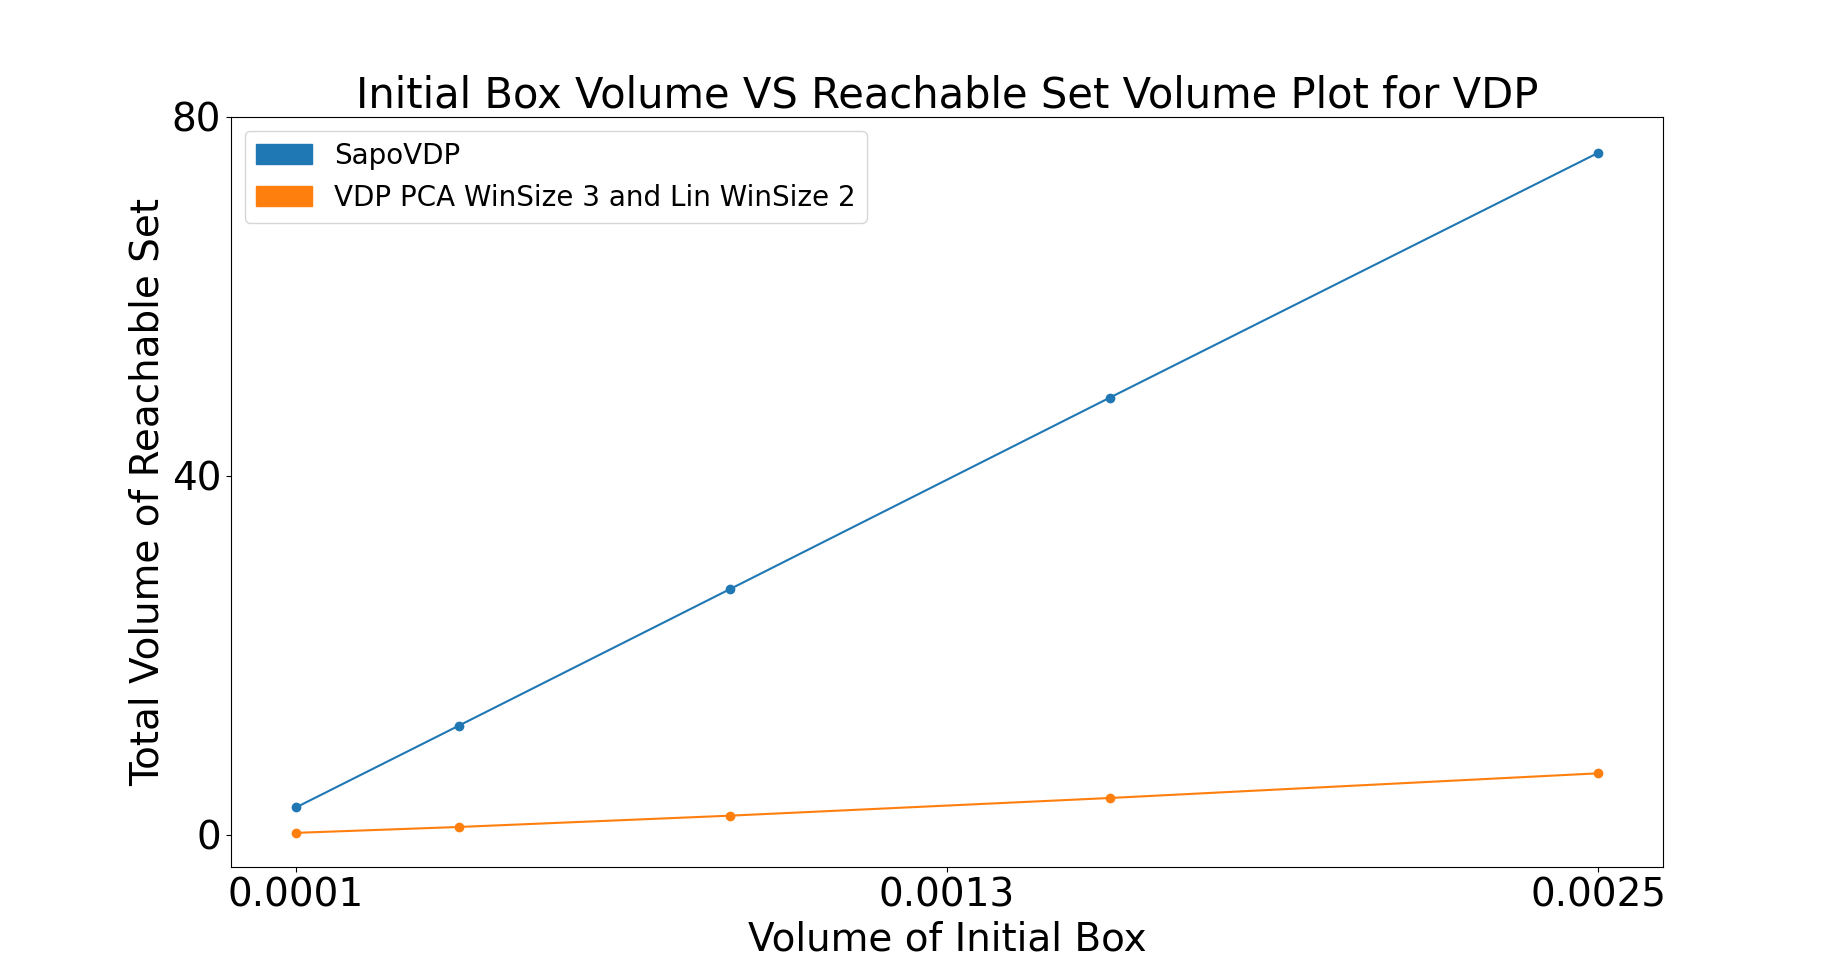
\includegraphics[width=1.1\textwidth, height=0.75\textwidth]{figures/InitVolVSReachVol/VDPInitReachVol.png}
    \caption{Vanderpol}
    \end{subfigure}%
    %\hspace{1em}
    \begin{subfigure}{0.5\textwidth}
    \centering
    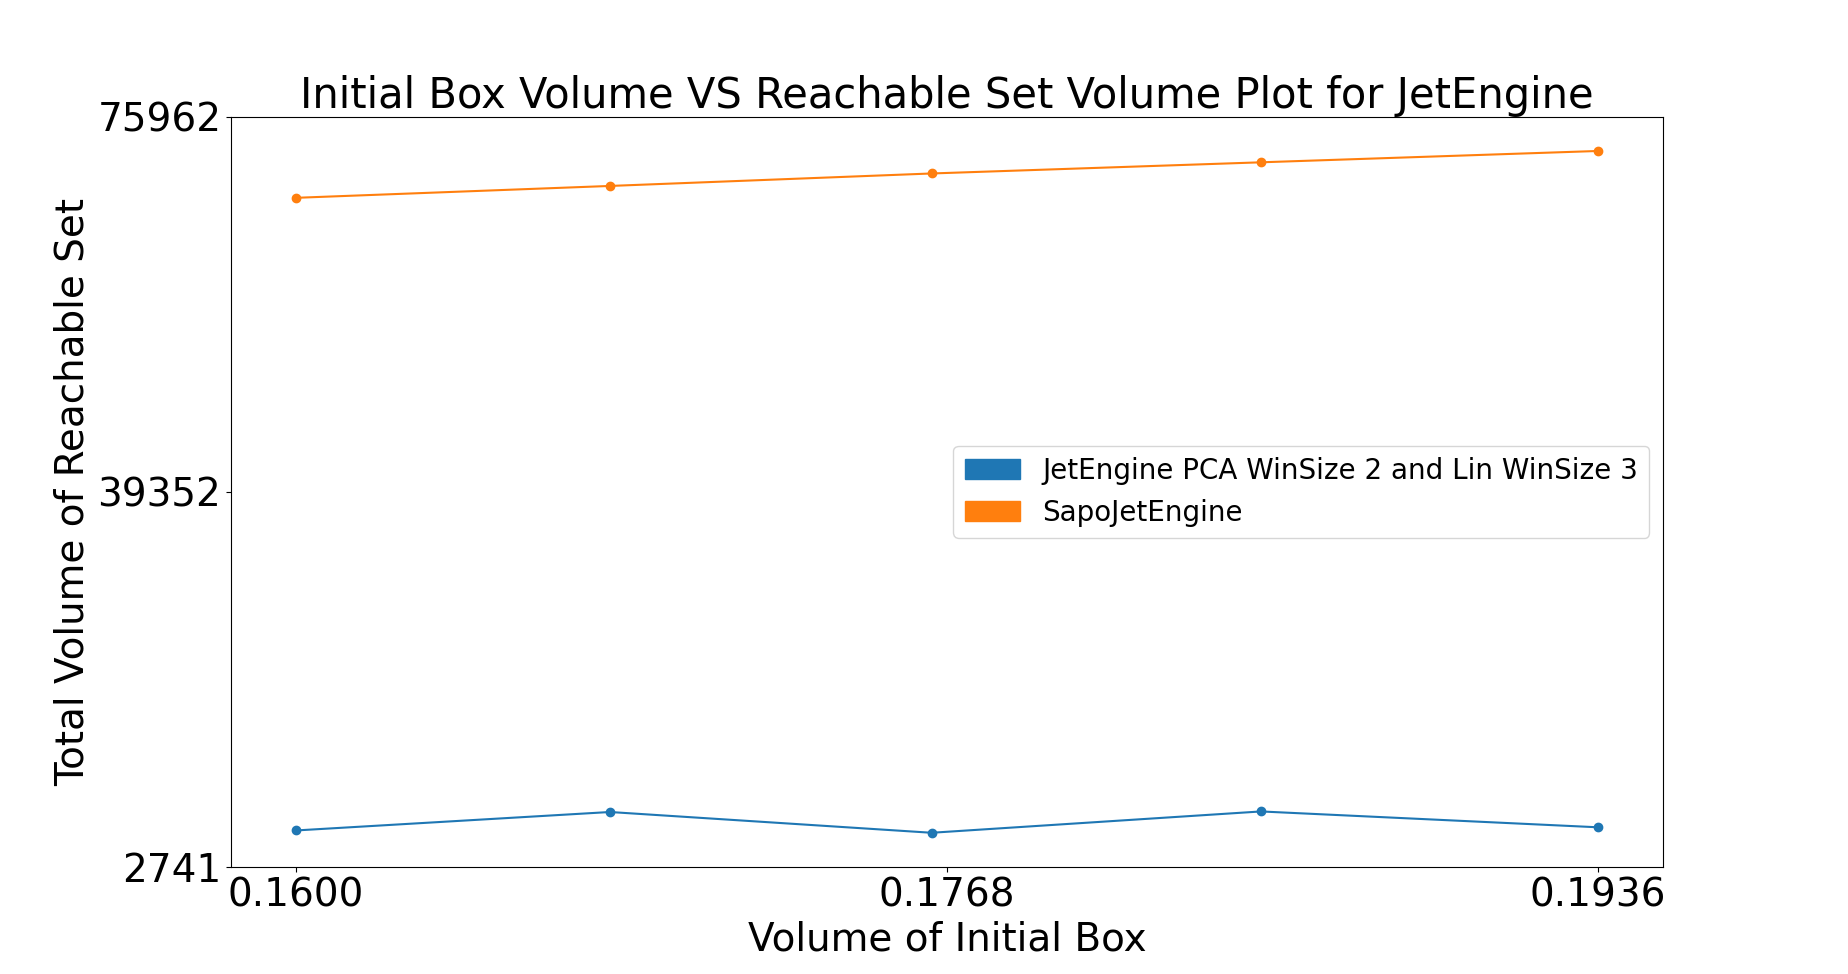
\includegraphics[width=1.1\textwidth, height=0.75\textwidth]{figures/InitVolVSReachVol/JetEngineInitReachVol.png}
    \caption{Jet Engine}
    \end{subfigure}

    \hspace{-1.5em}
    \begin{subfigure}{0.5\textwidth}
    \centering
    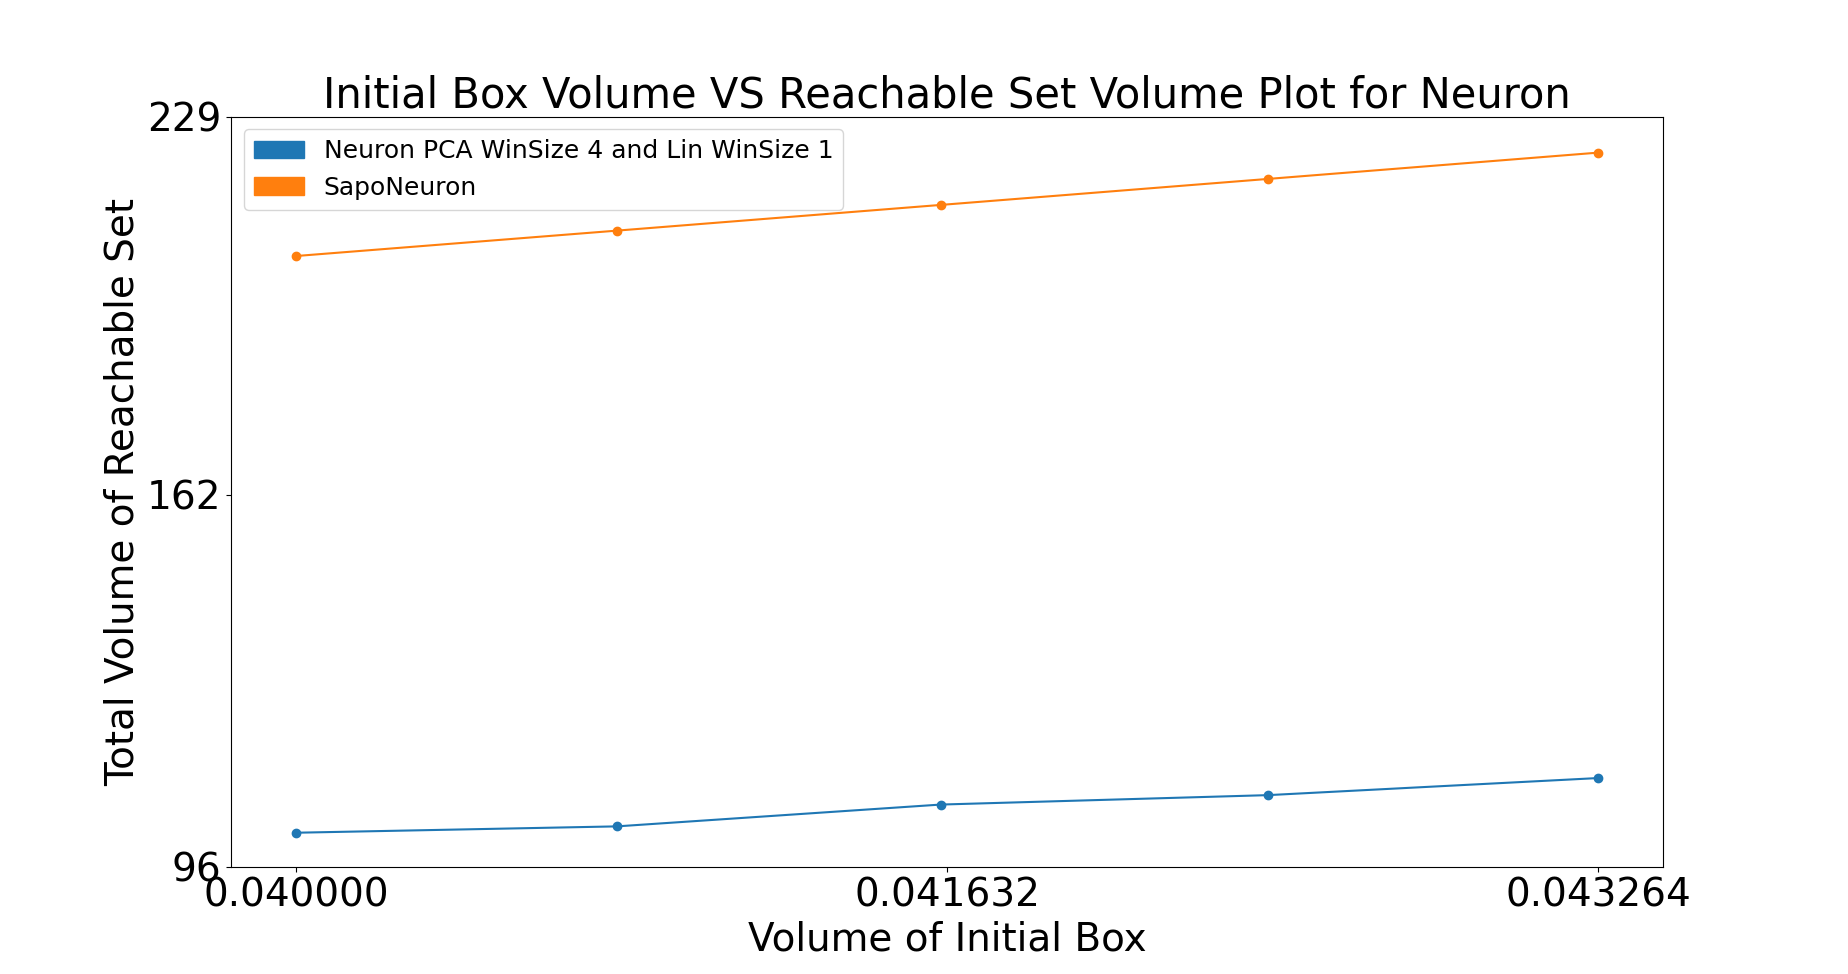
\includegraphics[width=1.1\textwidth, height=0.75\textwidth]{figures/InitVolVSReachVol/NeuronInitReachVol200steps.png}
    \caption{Neuron}
    \end{subfigure}%
    %\hspace{1em}
    \begin{subfigure}{0.5\textwidth}
    \centering
    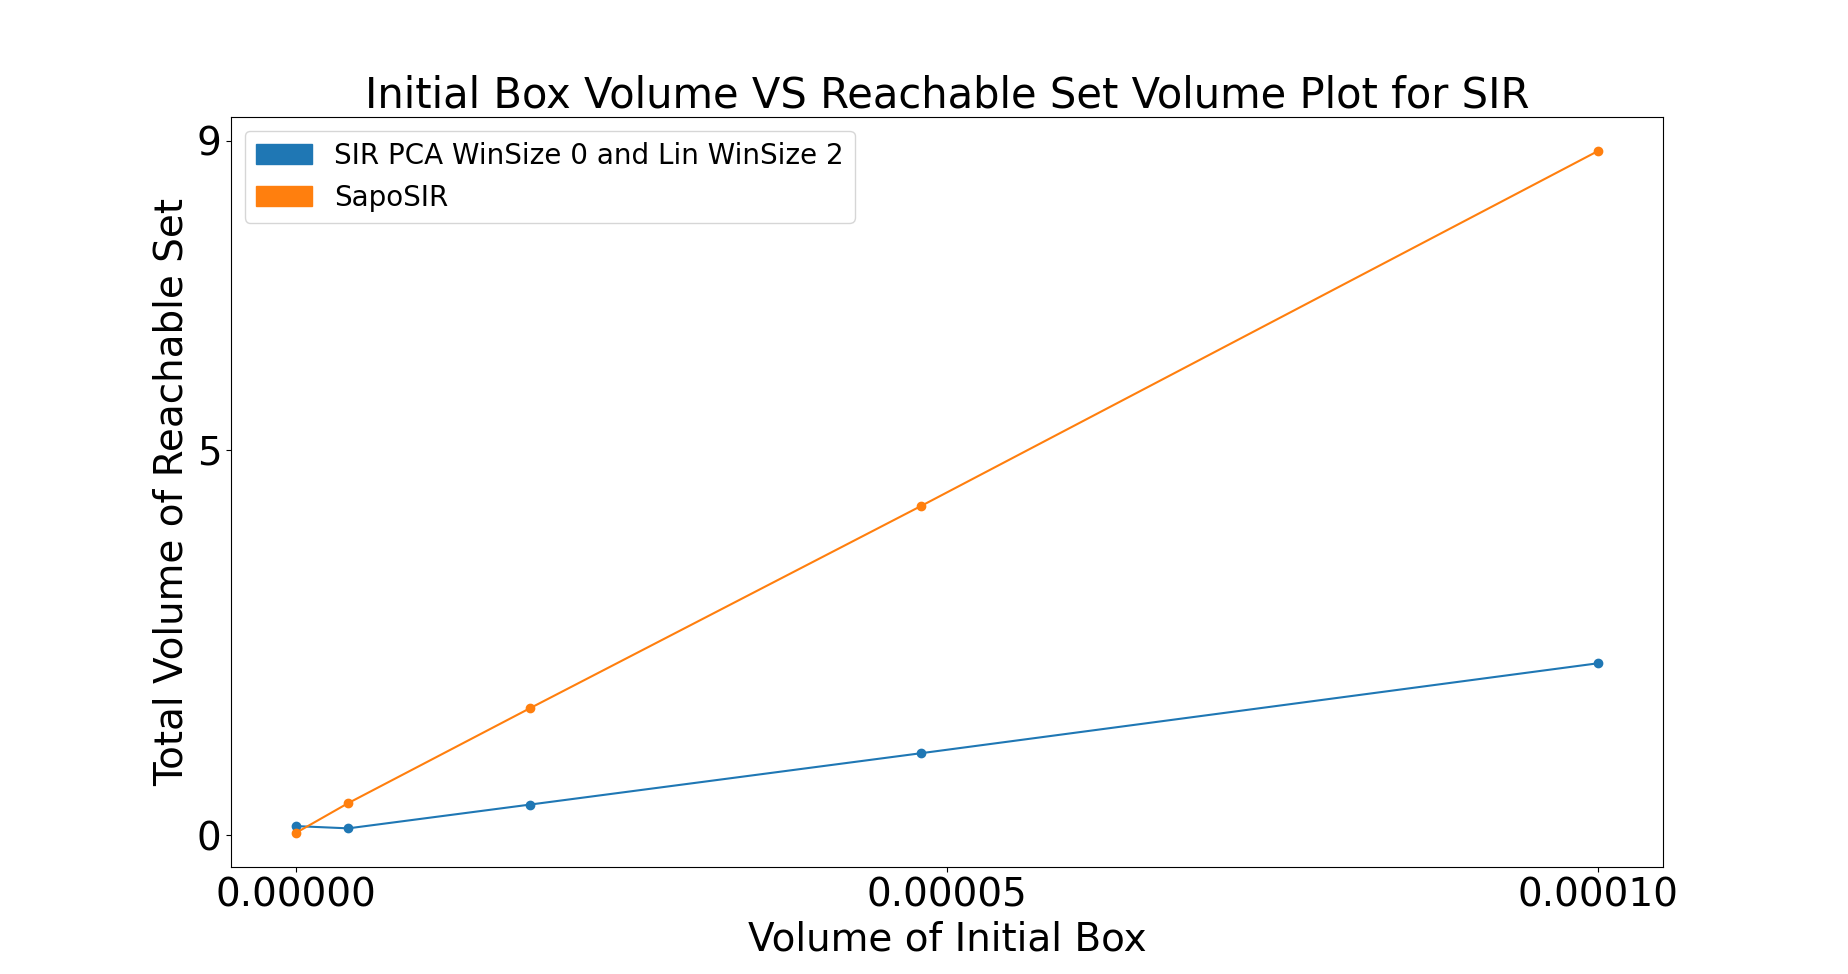
\includegraphics[width=1.1\textwidth, height=0.75\textwidth]{figures/InitVolVSReachVol/SIRInitReachVol.png}
    \caption{SIR}
    \end{subfigure}

    \hspace{-1.5em}
    \begin{subfigure}{0.5\textwidth}
    \centering
    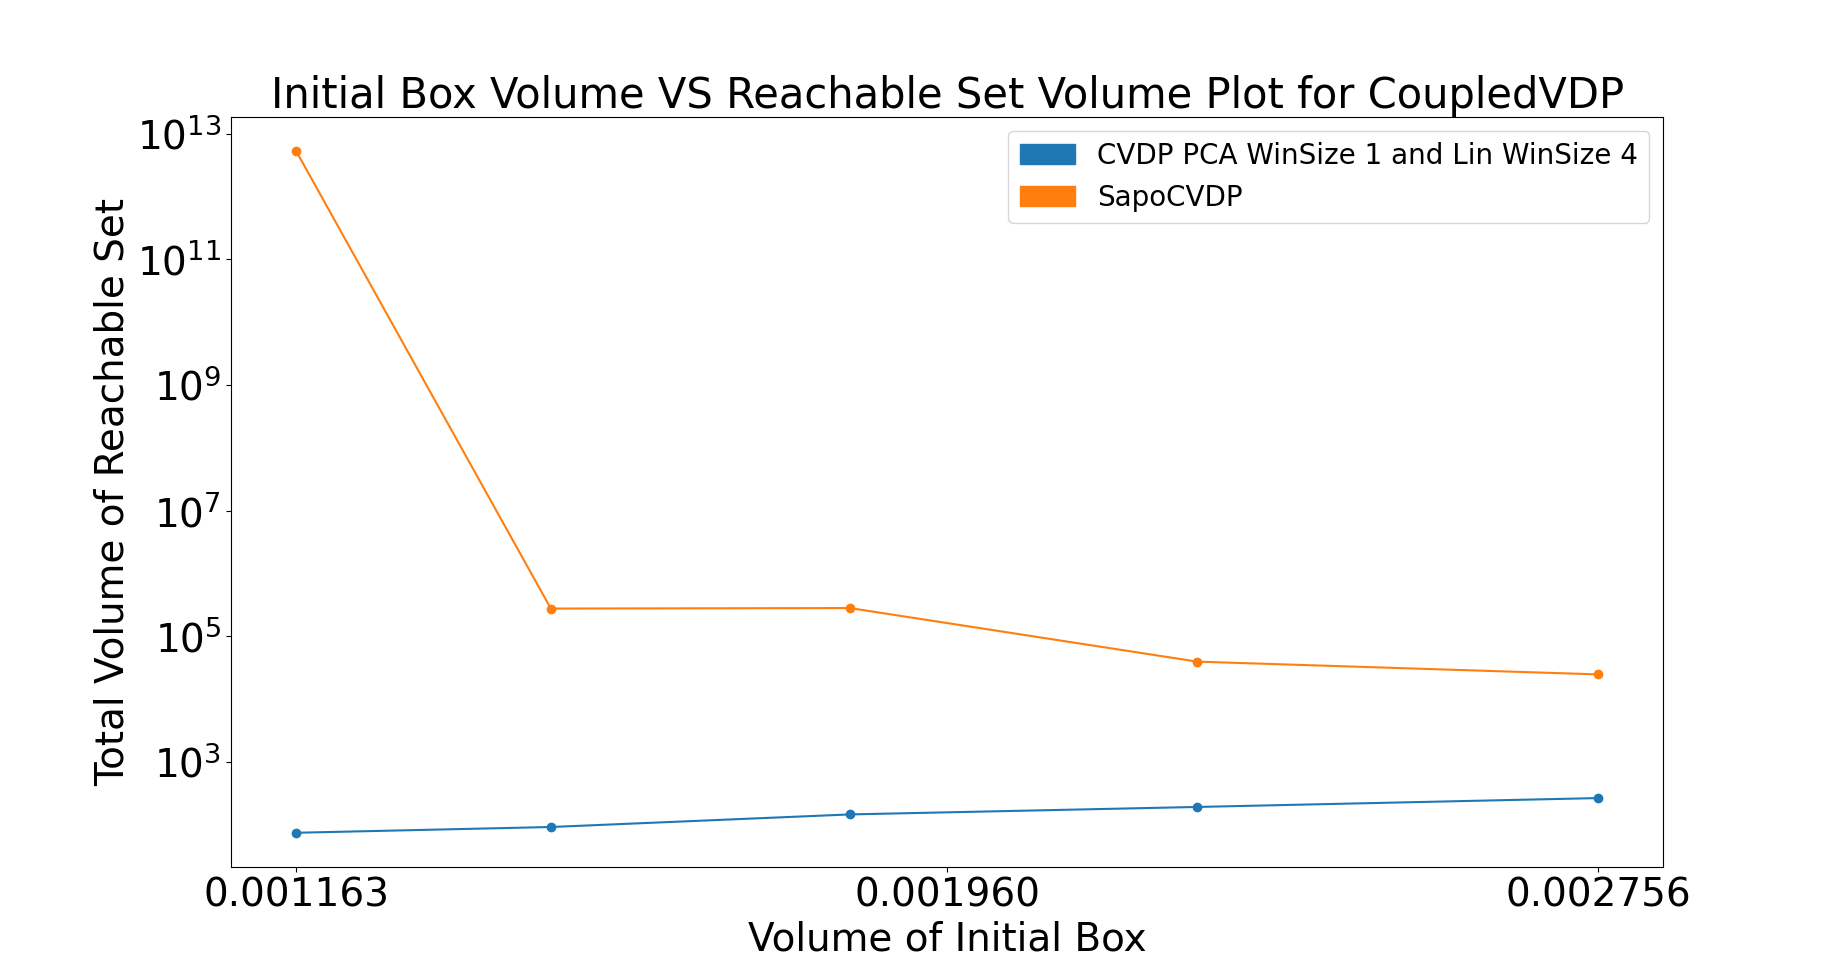
\includegraphics[width=1.1\textwidth, height=0.75\textwidth]{figures/InitVolVSReachVol/CVDPInitReachVol.png}
    \caption{Coupled Vanderpol}
    \end{subfigure}%
    %\hspace{1em}
    \begin{subfigure}{0.5\textwidth}
    \centering
    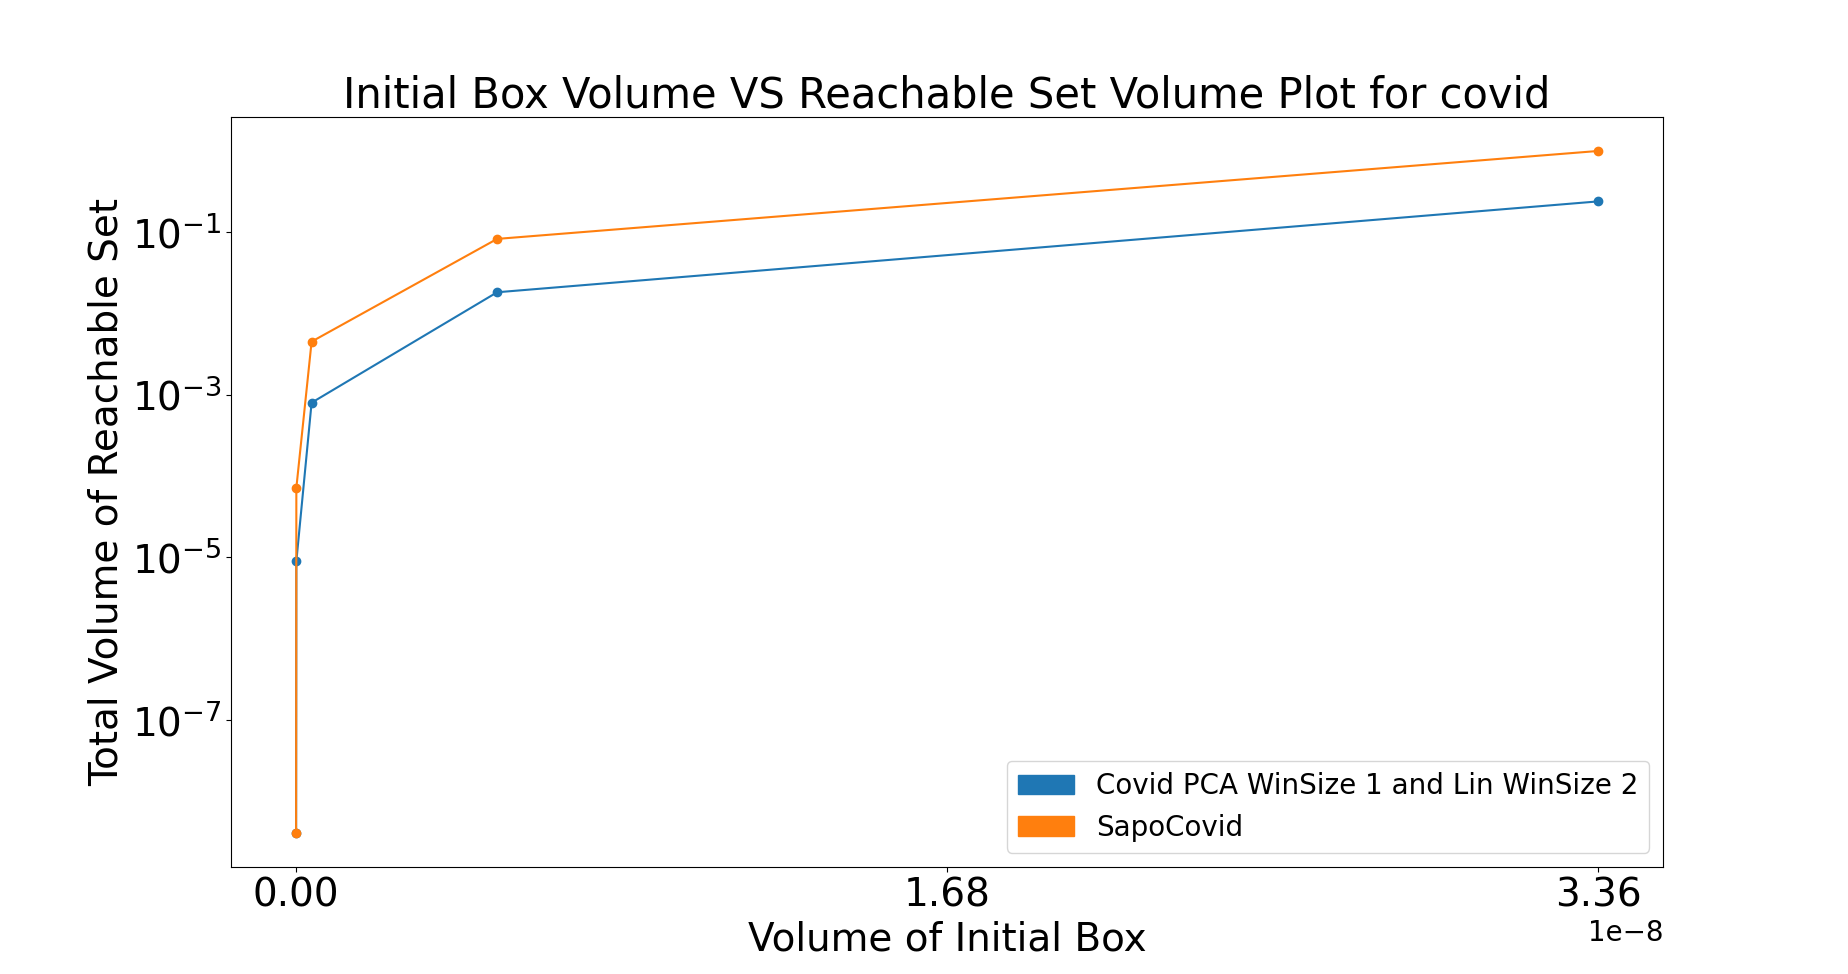
\includegraphics[width=1.1\textwidth, height=0.75\textwidth]{figures/InitVolVSReachVol/CovidInitReachVol.png}
    \caption{COVID}
    \end{subfigure}

    \caption{Comparison between the performance of diagonal static parallelotope bundles and that of the best performing dynamic parallelotope bundles as the volume of the initial set grows.}
    \label{fig:InitVolReachComp}
\end{figure}
\newpage

\begin{figure}[h!]
    \hspace{-1.5em}
    \begin{subfigure}{0.5\textwidth}
    \centering
    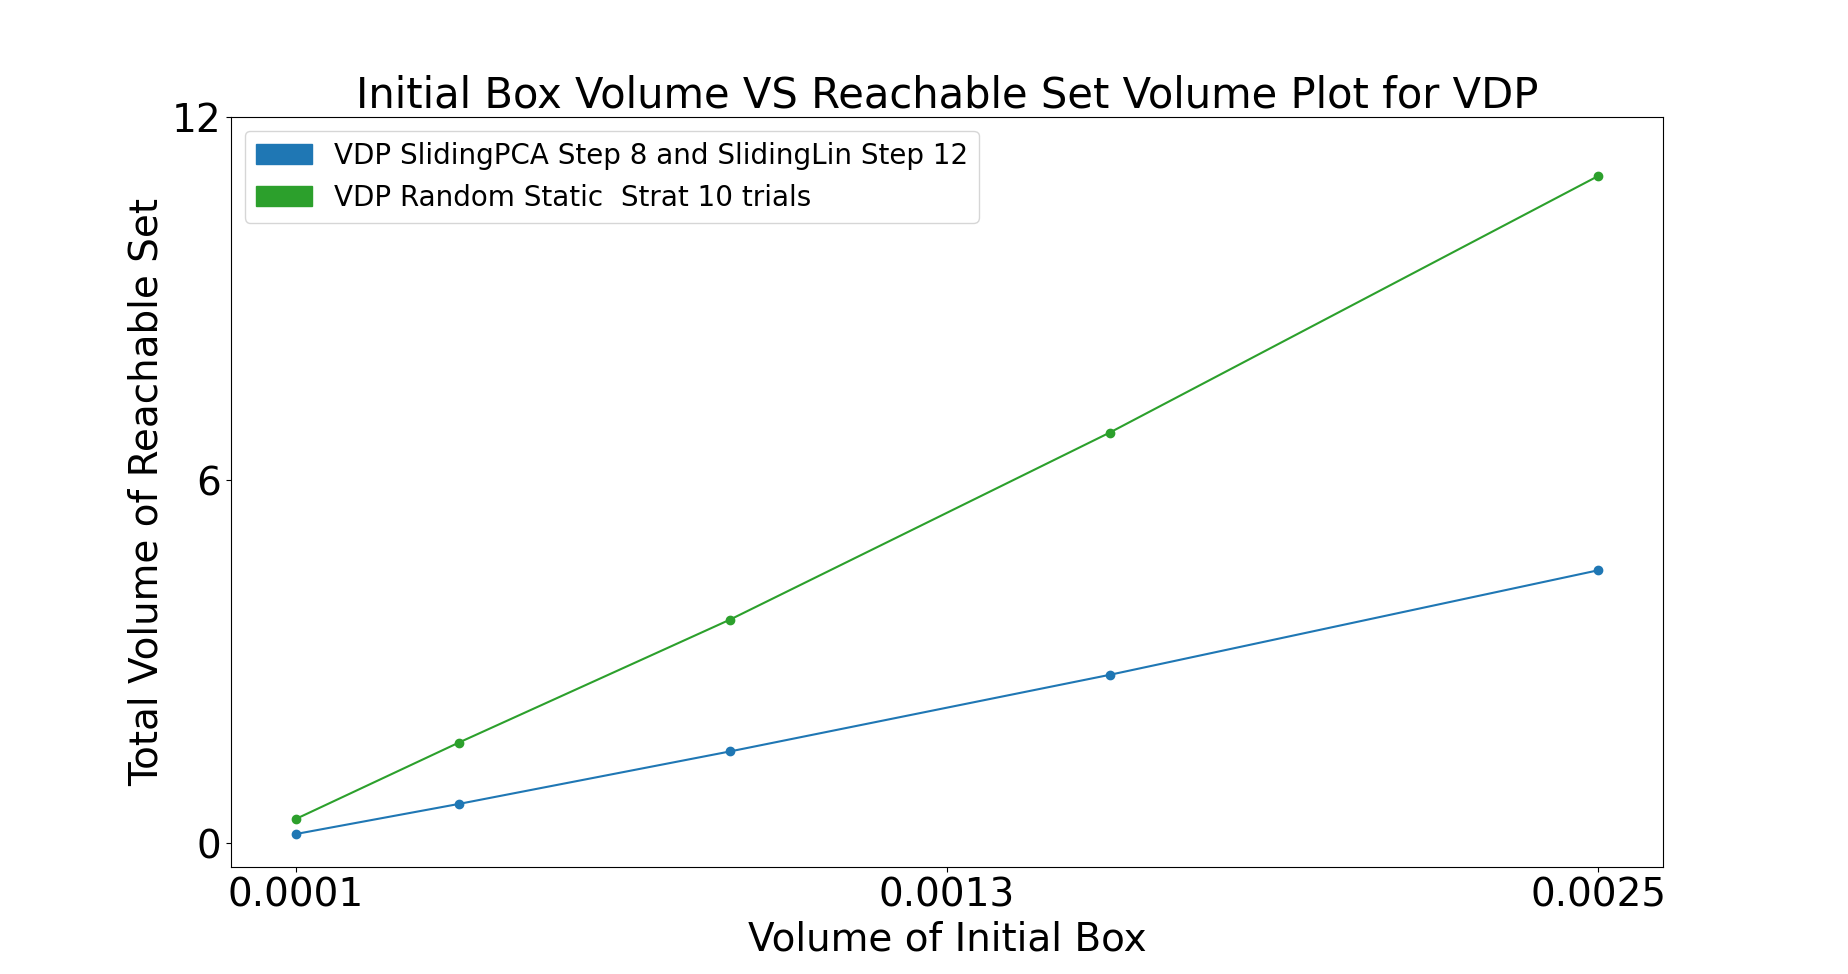
\includegraphics[width=1.1\textwidth, height=0.75\textwidth]{figures/InitVolVSReachVol/VDPInitReachVolRanStrat.png}
    \caption{Vanderpol}
    \end{subfigure}%
    \begin{subfigure}{0.5\textwidth}
    \centering
    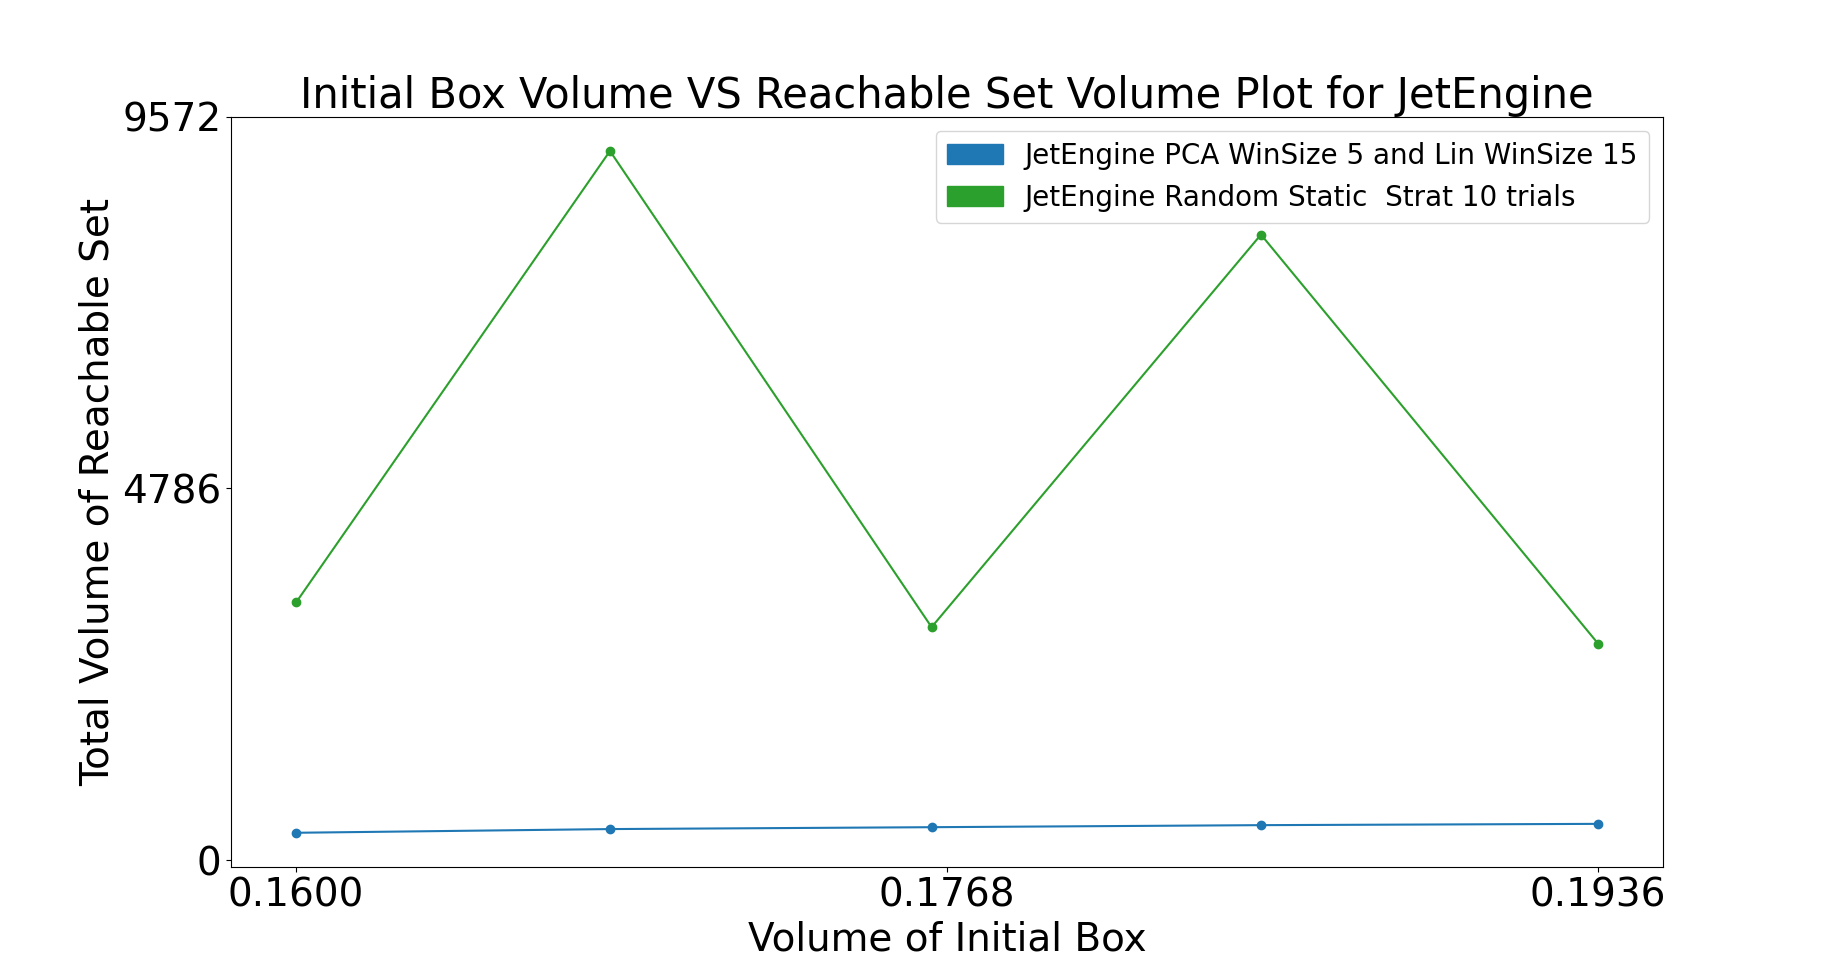
\includegraphics[width=1.1\textwidth, height=0.75\textwidth]{figures/InitVolVSReachVol/JetEngineInitReachVolRanStrat.png}
    \caption{Jet Engine}
    \end{subfigure}

    \hspace{-1.5em}
    \begin{subfigure}{0.5\textwidth}
    \centering
    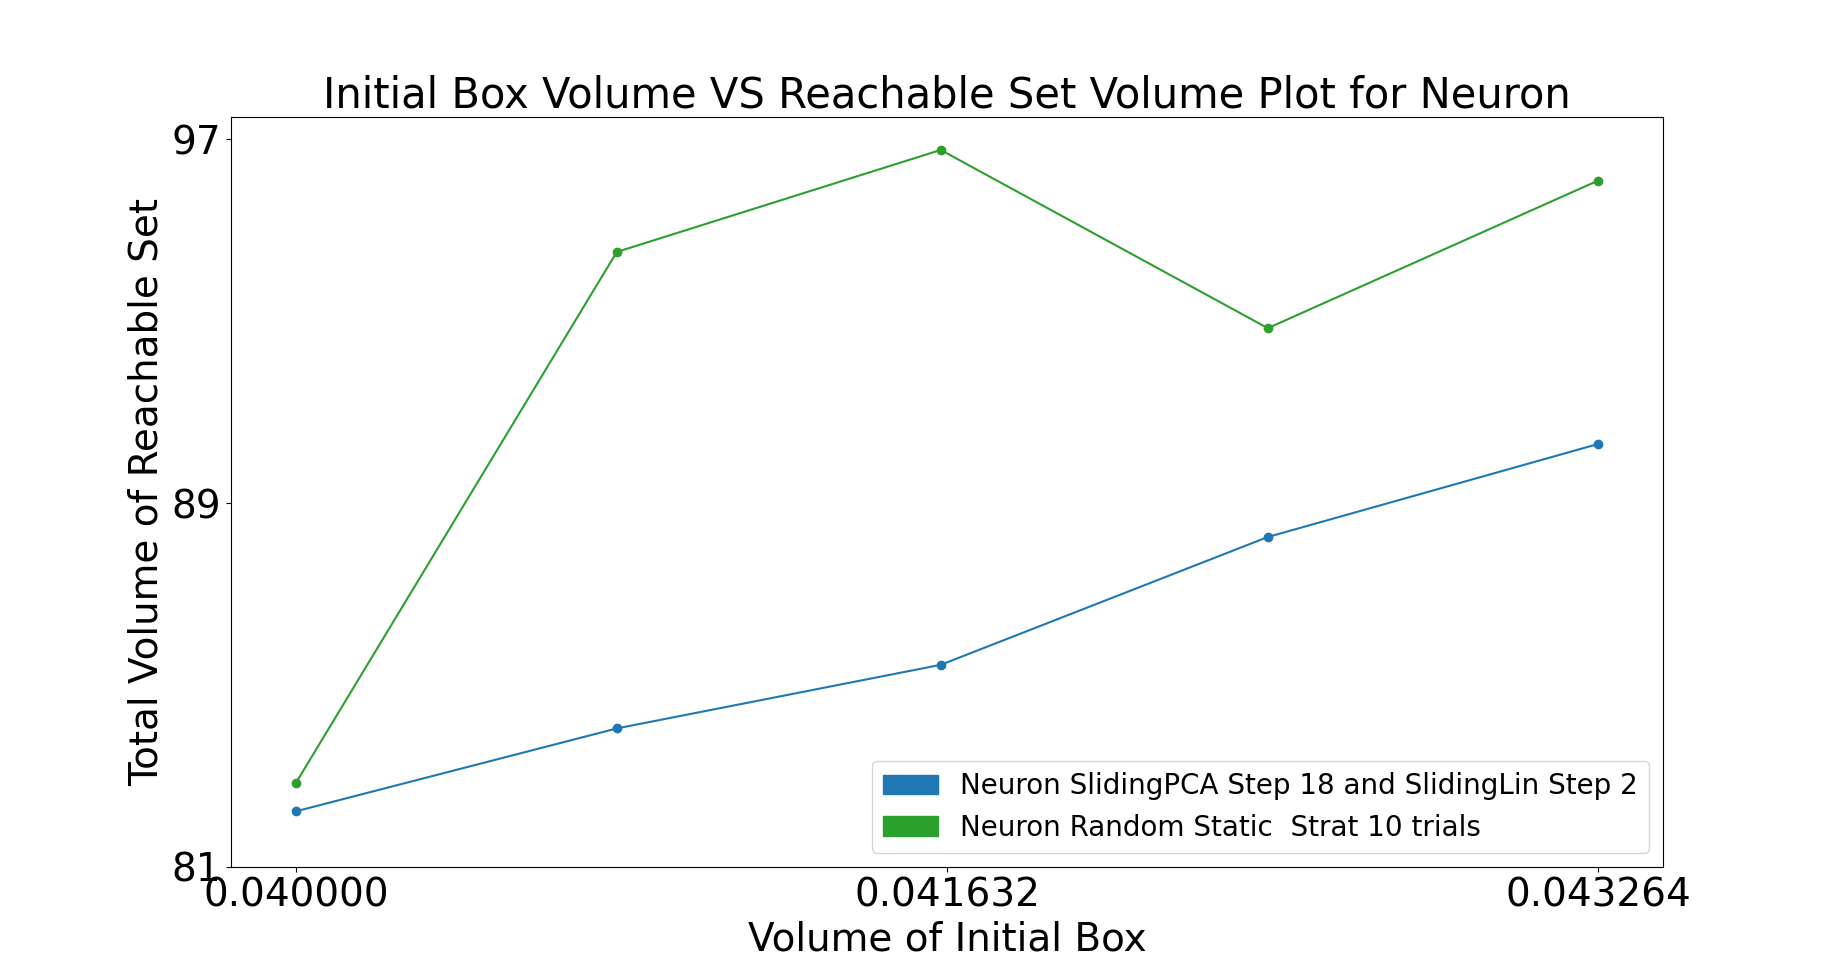
\includegraphics[width=1.1\textwidth, height=0.75\textwidth]{figures/InitVolVSReachVol/NeuronInitReachVolRanStrat.png}
    \caption{Neuron}
    \end{subfigure}%
    \begin{subfigure}{0.5\textwidth}
    \centering
    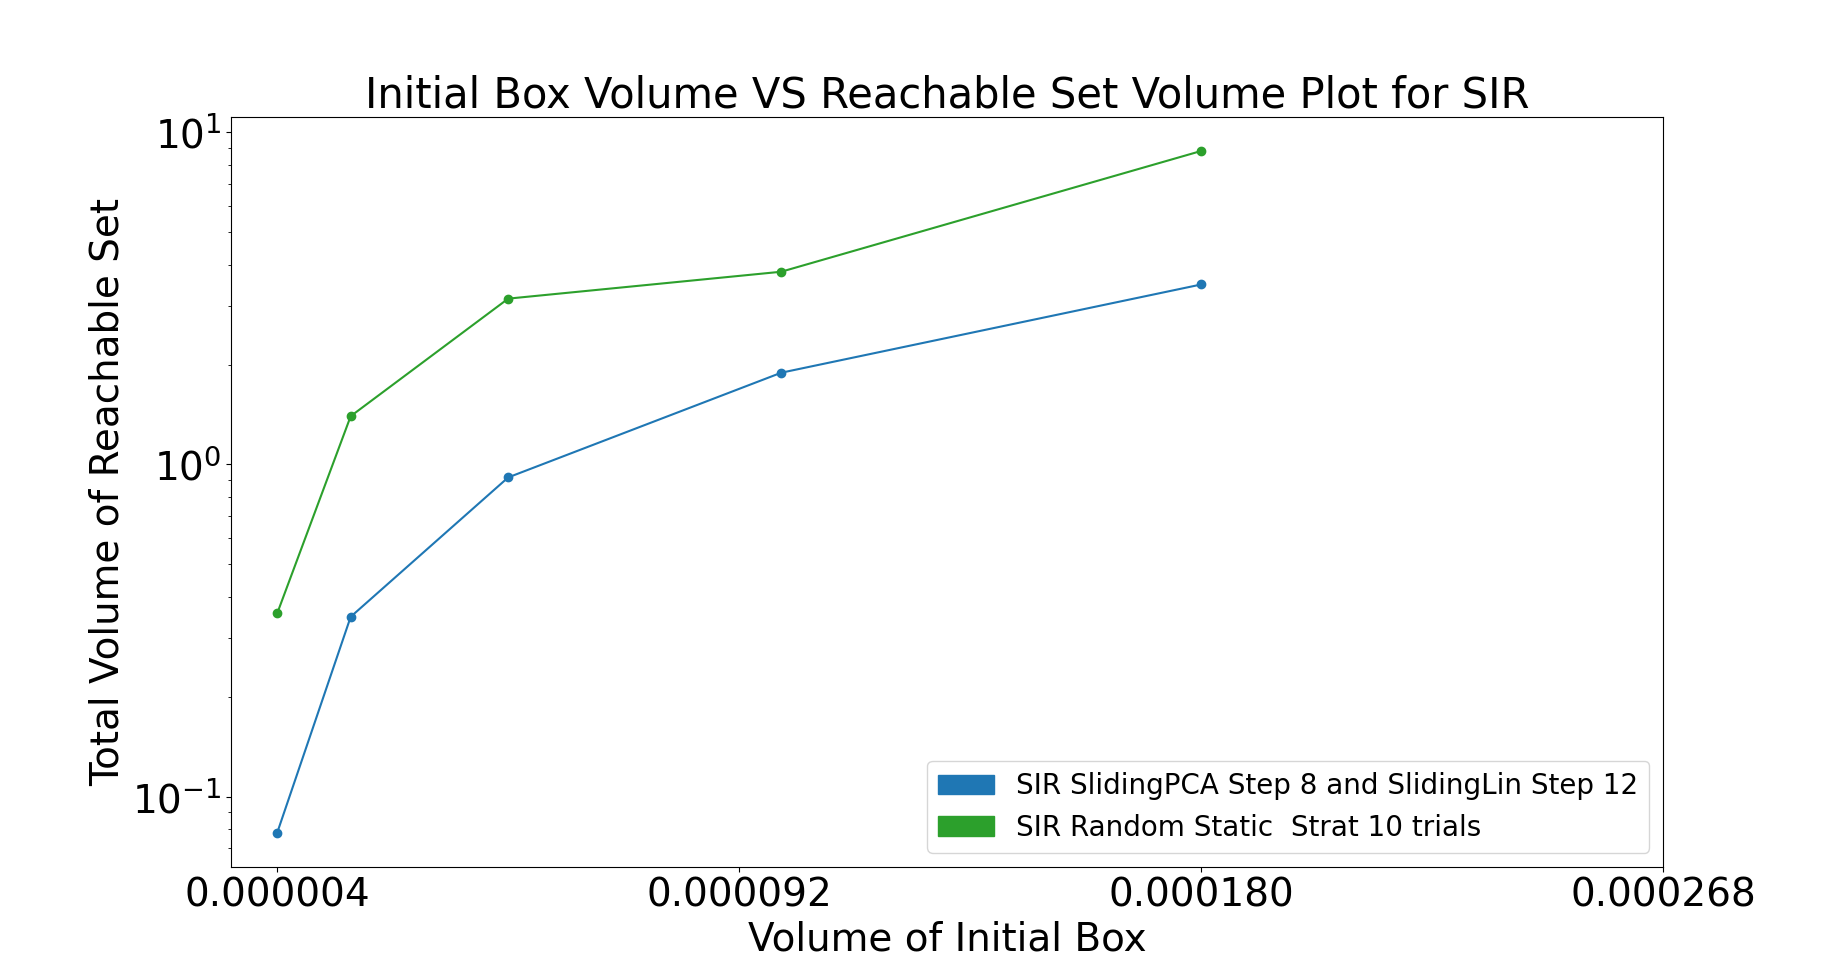
\includegraphics[width=1.1\textwidth, height=0.75\textwidth]{figures/InitVolVSReachVol/SIRInitReachVolRanStrat.png}
    \caption{SIR}
    \end{subfigure}

    \hspace{-1.5em}
    \begin{subfigure}{0.5\textwidth}
    \centering
    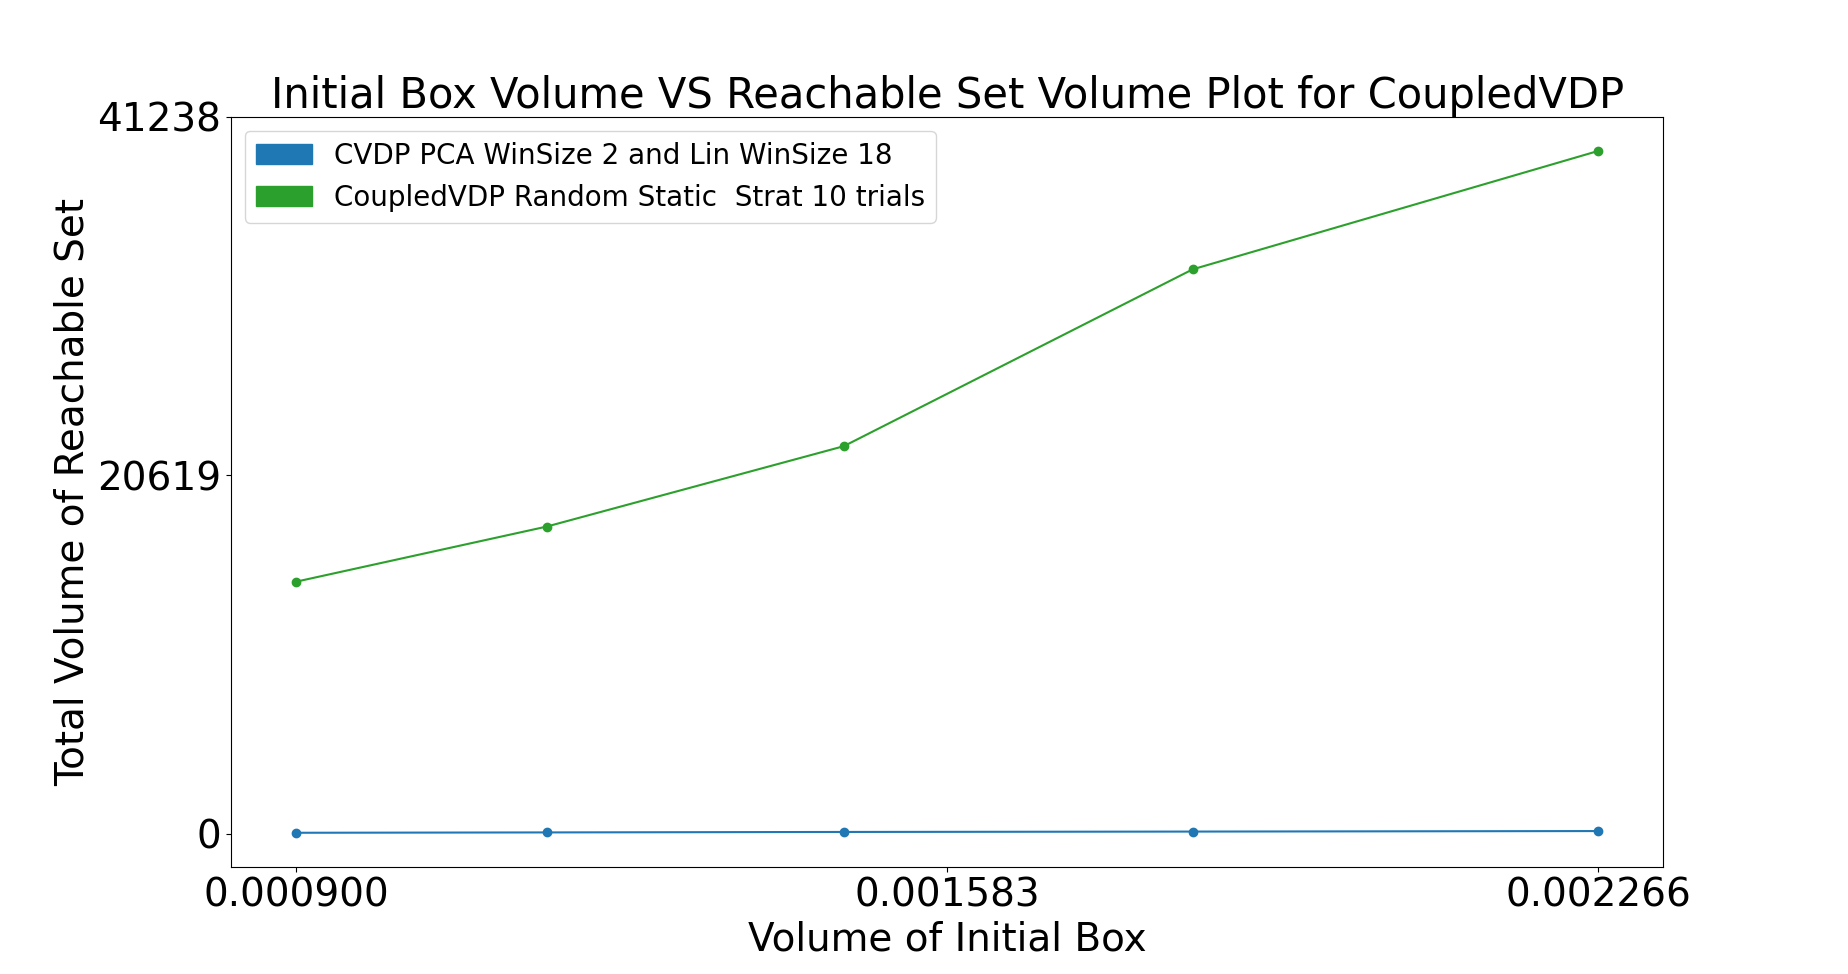
\includegraphics[width=1.1\textwidth, height=0.75\textwidth]{figures/InitVolVSReachVol/CVDPInitReachVolRanStrat.png}
    \caption{Coupled Vanderpol}
    \end{subfigure}%
    \begin{subfigure}{0.5\textwidth}
    \centering
    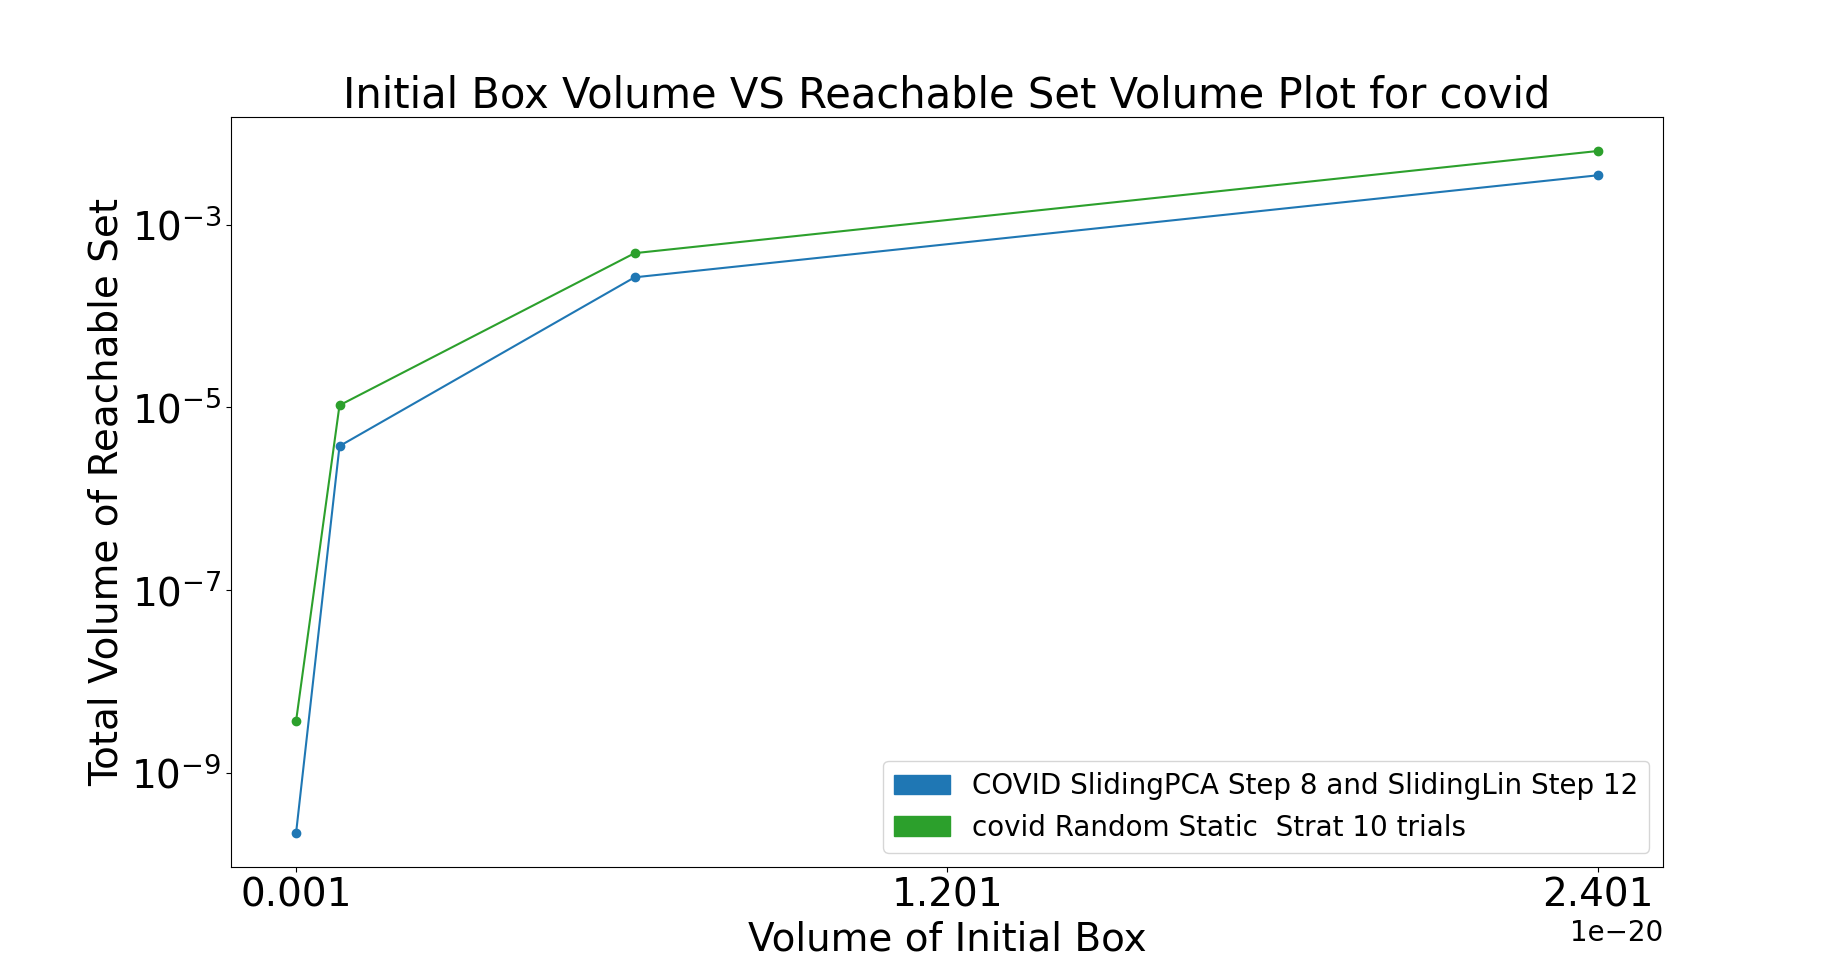
\includegraphics[width=1.1\textwidth, height=0.75\textwidth]{figures/InitVolVSReachVol/CovidInitReachVolRanStrat.png}
    \caption{COVID}
    \end{subfigure}

    \caption{Comparision between random static strategies and the best performing dynamic strategies as the volume of the initial set grows. The total reachable set volumes for random static strategies are averaged over ten trials for each system.}
    \label{fig:RanStaticStratComp}
\end{figure}
\newpage
